% main.tex -- report: training dynamics of tree tensor networks.
%
% Build with ./build.sh (pdflatex, bibtex, pdflatex, pdflatex); see README.md.
% One file per section in sections/; notation in macros.tex; TikZ sources in tikz/;
% figures collected from experiments/*/results/ into figures/ by collect_figures.sh.

\documentclass[11pt,letterpaper]{article}

% ---- fonts and page ------------------------------------------------------------------------
\usepackage[T1]{fontenc}
\usepackage[utf8]{inputenc}
\usepackage{lmodern}
\usepackage[margin=1in]{geometry}      % 6.5in x 9in text block
\usepackage[expansion=false]{microtype} % font expansion dropped a caption line (figure QA)

% ---- mathematics ---------------------------------------------------------------------------
\usepackage{amsmath,amssymb,amsthm}
\usepackage{mathtools}
\usepackage{bm}

% ---- figures, tables, colour -----------------------------------------------------------------
\usepackage{graphicx}
\graphicspath{{figures/}}
\usepackage{booktabs}
\usepackage{array}
\usepackage{tabularx}
\usepackage{xltabular}                  % multi-page tables with X columns (Appendix C)
\usepackage[dvipsnames]{xcolor}
\usepackage{siunitx}
\usepackage{caption}
\usepackage{subcaption}
\usepackage{tikz}
\usetikzlibrary{calc}
\usepackage{enumitem}
\usepackage{xspace}
\usepackage{aliascnt}
% Uncomment when an algorithm is needed (must stay before hyperref):
% \usepackage[ruled,vlined]{algorithm2e}

\captionsetup{font=small,labelfont=bf}
\captionsetup[sub]{font=small,labelfont=bf}
\sisetup{separate-uncertainty=true}
\setlist{itemsep=2pt,topsep=4pt}

% ---- bibliography and links (hyperref, doi and cleveref come last) ----------------------------
\usepackage[round,authoryear]{natbib}
\bibliographystyle{plainnat}
\usepackage[colorlinks=true,linkcolor=MidnightBlue,citecolor=OliveGreen,urlcolor=RoyalPurple,
            bookmarksnumbered=true]{hyperref}
\usepackage{doi}
\usepackage[capitalise,noabbrev]{cleveref}
\hypersetup{pdftitle={Training dynamics of tree tensor networks},
            pdfsubject={Saddle-to-saddle, lazy and rich regimes of tree tensor network training}}

% ---- theorem-like environments ------------------------------------------------------------------
% One shared counter, numbered within sections. Each environment gets its own alias of the
% "theorem" counter: with the current LaTeX kernel, cleveref (v0.21.4) would otherwise call every
% environment that shares a counter a "Theorem". The environment "conjecture" is completed below,
% after the status tags, because its name is shared with the \conjecture tag.
\newcommand{\newsharedtheorem}[2]{% #1 environment, #2 printed name
  \newaliascnt{#1}{theorem}\newtheorem{#1}[#1]{#2}\aliascntresetthe{#1}%
  \crefname{#1}{#2}{#2s}}
\theoremstyle{plain}
\newtheorem{theorem}{Theorem}[section]
\crefname{theorem}{Theorem}{Theorems}
\newsharedtheorem{proposition}{Proposition}
\newsharedtheorem{lemma}{Lemma}
\newsharedtheorem{corollary}{Corollary}
\crefname{corollary}{Corollary}{Corollaries}
\newsharedtheorem{conjectureenv}{Conjecture}
\theoremstyle{definition}
\newsharedtheorem{definition}{Definition}
\theoremstyle{remark}
\newsharedtheorem{remark}{Remark}

% ---- status tags and new/known markers ---------------------------------------------------------
% Every claim carries one status tag:
%   \proven      complete proof given (or cited)
%   \derived     derivation under stated assumptions (not a full proof)
%   \empirical   supported by experiments only
%   \conjecture  stated without derivation or sufficient evidence
% Results are marked \newresult[qualifier] (believed new) or \knownresult[reference] (known).
\definecolor{tagproven}{HTML}{1B7837}
\definecolor{tagderived}{HTML}{2166AC}
\definecolor{tagempirical}{HTML}{B35806}
\definecolor{tagconjecture}{HTML}{762A83}
\definecolor{tagnew}{HTML}{C51B7D}
\definecolor{tagknown}{HTML}{525252}
\definecolor{todocolor}{HTML}{B2182B}

\newcommand{\statustag}[2]{% #1 colour, #2 label
  {\setlength{\fboxsep}{1.1pt}\setlength{\fboxrule}{0.4pt}%
   \fcolorbox{#1}{#1!7}{\textcolor{#1}{\sffamily\scriptsize\bfseries #2}}}}
\newcommand{\tagnote}[1]{\if\relax\detokenize{#1}\relax\else\,{\upshape\small(#1)}\fi}
\DeclareRobustCommand{\proven}{\statustag{tagproven}{proven}}
\DeclareRobustCommand{\derived}{\statustag{tagderived}{derived}}
\DeclareRobustCommand{\empirical}{\statustag{tagempirical}{empirical}}
\DeclareRobustCommand{\conjecturetag}{\statustag{tagconjecture}{conjecture}}
\DeclareRobustCommand{\newresult}[1][]{\statustag{tagnew}{new}\tagnote{#1}}
\DeclareRobustCommand{\knownresult}[1][]{\statustag{tagknown}{known}\tagnote{#1}}
\let\conjecture\conjecturetag

% \begin{conjecture}[title] ... \end{conjecture} is the theorem-like environment; elsewhere
% \conjecture is the status tag. The env/begin hook runs inside the environment's group just
% before \begin calls \conjecture, so the redefinition below is local to the environment and the
% tag is restored for the environment's body.
\AddToHook{env/conjecture/begin}{%
  \def\conjecture{\let\conjecture\conjecturetag\conjectureenv}%
  \let\endconjecture\endconjectureenv}

\pdfstringdefDisableCommands{%
  \def\proven{[proven]}\def\derived{[derived]}\def\empirical{[empirical]}%
  \def\conjecture{[conjecture]}\def\newresult{[new]}\def\knownresult{[known]}}

% ---- drafting aids ---------------------------------------------------------------------------
% \showtodosfalse hides all placeholders and TODO notes (for a final version).
\newif\ifshowtodos
\showtodostrue
\newcommand{\placeholder}[1]{%
  \ifshowtodos\par\noindent{\color{todocolor}\small\itshape[#1]}\par\fi}
\newcommand{\TODO}[1]{\ifshowtodos{\color{todocolor}\sffamily\footnotesize[TODO: #1]}\fi}

% ---- notation ---------------------------------------------------------------------------------
% macros.tex -- notation used throughout the report.
%
% Conventions follow notes/model.md and notes/diagnostics.md. Change a symbol here, not in the
% sections. Symbols that clash with the notes are renamed here on purpose:
%   - the tangent kernel is \TK (Theta), because K is the number of cores (the notes call it K_t);
%   - aligned-init amplitudes are q_{v,r} (\amp), because a_r is the teacher-component overlap;
%   - the gradient-flow preconditioner is diag(eta) (\Pre), because D is the set of differing sites;
%   - the rooted tree is blackboard T, because \mathcal{T}(Z) is the first-escape prefactor;
%   - event widths are omega_r, because w is the weight ratio s_2/s_1.

% ---- general ---------------------------------------------------------------------------------
\newcommand{\R}{\mathbb{R}}
\newcommand{\E}{\mathbb{E}}
\newcommand{\Normal}{\mathcal{N}}
\newcommand{\T}{^{\top}}                          % transpose
\newcommand{\Id}{I}                               % identity matrix
\newcommand{\iid}{i.i.d.\@\xspace}
\DeclareMathOperator{\tr}{tr}
\DeclareMathOperator{\rank}{rank}
\DeclareMathOperator{\diag}{diag}
\DeclareMathOperator{\GL}{GL}
\DeclareMathOperator*{\argmin}{arg\,min}
\DeclarePairedDelimiter{\abs}{\lvert}{\rvert}
\DeclarePairedDelimiter{\norm}{\lVert}{\rVert}
\DeclarePairedDelimiterX{\ip}[2]{\langle}{\rangle}{#1,\,#2}
\newcommand{\normF}[1]{\norm{#1}_{F}}             % Frobenius norm
\newcommand{\normmax}[1]{\norm{#1}_{\max}}        % largest absolute entry
\newcommand{\ipS}[2]{\ip{#1}{#2}_{\Sig}}          % Sigma-weighted inner product
\newcommand{\normS}[1]{\norm{#1}_{\Sig}}          % Sigma-weighted norm
\newcommand{\dd}{\mathrm{d}}                      % differential
\newcommand{\ddt}{\frac{\dd}{\dd t}}

% ---- inputs and data ---------------------------------------------------------------------------
\newcommand{\Ns}{N}                               % number of sites
\newcommand{\pd}[1][]{d_{#1}}                     % physical (local feature) dimension of site i
\newcommand{\xs}[1]{x^{(#1)}}                     % input at site i
\newcommand{\feat}[1]{\phi_{#1}}                  % local feature map of site i
\newcommand{\Feat}{\Phi}                          % product feature tensor
\newcommand{\Sig}{\Sigma}                         % product covariance Sigma_1 (x) ... (x) Sigma_N
\newcommand{\Sigi}[1]{\Sigma_{#1}}                % covariance of site i
\newcommand{\nsamp}{n}                            % training-set size
\newcommand{\batch}{B}                            % minibatch size
\newcommand{\nprobe}{P}                           % size of the kernel probe set

% ---- tree and tensor network ---------------------------------------------------------------------
\newcommand{\tree}{\mathbb{T}}                    % rooted tree (\mathcal{T}(Z) is the first-escape prefactor)
\newcommand{\nodes}{\mathcal{V}}                  % its nodes (= cores)
\newcommand{\edges}{\mathcal{E}}                  % its edges (= bonds)
\newcommand{\Kc}{K}                               % number of cores
\newcommand{\vroot}{\mathrm{root}}                % the root node
\newcommand{\pa}[1]{p(#1)}                        % parent of node v
\newcommand{\ch}[1]{\mathrm{ch}(#1)}              % children of node v
\newcommand{\sites}[1]{S_{#1}}                    % sites attached to node v
\newcommand{\below}[1]{A_{#1}}                    % sites in the subtree below node v
\newcommand{\edge}[1]{e_{#1}}                     % edge between node v and its parent
\newcommand{\G}[1]{G_{#1}}                        % core of node v
\newcommand{\Gm}[2]{G_{#1,(#2)}}                  % core v matricized with its e-leg as rows
\newcommand{\bd}[1]{\chi_{#1}}                    % bond dimension of edge e_v
\newcommand{\fanin}[1]{F_{#1}}                    % fan-in of core v
\newcommand{\params}{\theta}                      % all parameters (cores)
\newcommand{\W}{W}                                % tensor represented by the TTN
\newcommand{\Wt}{W^{*}}                           % teacher tensor
\newcommand{\Wz}{W_{0}}                           % tensor at initialization
\newcommand{\mat}[2]{#1^{\langle #2\rangle}}      % matricization of a tensor across edge e
\newcommand{\Sub}[1]{T_{#1}}                      % contraction of the subtree below v

% ---- initialization ------------------------------------------------------------------------------
\newcommand{\isc}{\sigma}                         % per-core init scale
\newcommand{\iscv}[1]{\sigma_{#1}}                % init scale of core v
\newcommand{\fsc}{\alpha}                         % function-space init scale sigma^K
\newcommand{\amp}[2]{q_{#1,#2}}                   % aligned-init amplitude of core v on component r
\newcommand{\prodamp}[1]{\Pi_{#1}}                % product of amplitudes of component r

% ---- teacher -------------------------------------------------------------------------------------
\newcommand{\ncomp}{R}                            % number of CP components
\newcommand{\tw}[1]{s_{#1}}                       % teacher weight of component r
\newcommand{\fac}[2]{u_{#1}^{(#2)}}               % factor of component r at site i
\newcommand{\U}[1]{U_{#1}}                        % rank-one term of component r (unit norm)
\newcommand{\ov}[1]{a_{#1}}                       % overlap with teacher component r
\newcommand{\Lpart}[1]{L_{#1}}                    % partial-fit loss level

% ---- bond spectra --------------------------------------------------------------------------------
\newcommand{\bs}[2]{s^{#1}_{#2}}                  % k-th singular value across edge e
\newcommand{\bst}[2]{s^{#1,*}_{#2}}               % same for the teacher
\newcommand{\rk}[1]{\operatorname{rk}_{#1}}       % effective bond rank of edge e
\newcommand{\rkH}[1]{\operatorname{rk}^{H}_{#1}}  % entropy rank of edge e

% ---- training ------------------------------------------------------------------------------------
\newcommand{\Loss}{L}                             % population loss
\newcommand{\Lemp}{\hat{L}_{\nsamp}}              % empirical loss
\newcommand{\lr}{\eta}                            % learning rate (step size) of GD/SGD
\newcommand{\lrm}[1]{\eta_{#1}}                   % per-core learning-rate multiplier
\newcommand{\mask}{\mathfrak{m}}                  % 0/1 gradient mask (m is |V_D|)
\newcommand{\Pre}{\operatorname{diag}(\boldsymbol{\eta})} % diagonal preconditioner (per-entry rates and mask); D is the site set
\newcommand{\tmax}{t_{\max}}

% ---- symmetries ------------------------------------------------------------------------------
\newcommand{\Q}[1]{Q_{#1}}                        % conserved quantity of bond e

% ---- diagnostics ---------------------------------------------------------------------------------
\newcommand{\TK}{\Theta}                          % tangent kernel (tensor kernel; restricted to the probe set where stated)
\newcommand{\dTK}{\delta_{\TK}}                   % relative kernel change
\newcommand{\dth}{\delta_{\params}}               % relative parameter change
\newcommand{\KTA}{\mathcal{A}}                    % kernel-target alignment
\newcommand{\Jac}{J}                              % Jacobian dW/dtheta
\newcommand{\Hess}{H}                             % Hessian of the loss
\newcommand{\Hperp}{H_{\perp}}                    % gauge-projected Hessian
\newcommand{\sep}[1]{\rho_{#1}}                   % separation ratio of consecutive events
\newcommand{\tev}[1]{t_{#1}}                      % event time
\newcommand{\wev}[1]{\omega_{#1}}                 % event width (w is the weight ratio)
\newcommand{\tmid}[1]{t^{\mathrm{mid}}_{#1}}      % plateau midpoint


% ---- front matter ---------------------------------------------------------------------------
\title{Training dynamics of tree tensor networks:\\
       saddle-to-saddle, lazy and rich regimes}
\author{TTN regimes project\thanks{Working draft; authors to be added.}}
\date{Draft of \today}

\begin{document}

\maketitle

\begin{abstract}
  \sloppy
  % At most 200 words. Status words (provably, confirmed) follow the tags of Sections 3-6.
  We study how gradient flow trains tree tensor networks,
  $f(x)=\langle W,\phi_0(x_0)\otimes\cdots\otimes\phi_{N-1}(x_{N-1})\rangle$ with $W$ contracted from $K$ cores on a
  tree, on a teacher's population loss. From small initialization (scale $\sigma$) it is
  saddle-to-saddle: it rests at fixed-rank critical points, and each escape raises the bond ranks along a
  route, a connected set of cores moving together; on large trees, routes often die first. The first
  plateau lasts $\propto\sigma^{-(K-2)}$, with a prefactor computed per initialization. Later the tree decides:
  the smallest route, of $k^*$ cores, gives no plateau ($k^*=1$), a logarithmic one ($k^*=2$) or one
  $\propto\sigma^{-(k^*-2)}$ (confirmed to $k^*=5$). With one learned component and a spare bond channel,
  $k^*$ is provably the saddle order under a spectral condition, met by two-component teachers learned in
  weight order; from $k^*=5$ on, non-strict saddles can have lower order. Non-orthogonal teachers make the next
  saddle strict on matrix product states, not on the binary and hierarchical Tucker trees tested, whose
  internal cores carry no site. The learning order is a race set by the initialization unless components
  differ on two cores only. Without the initial function, larger $\sigma$ leads through a rich regime to a
  lazy one, which needs every bond at its largest possible rank.
\end{abstract}

\tableofcontents

\paragraph{Conventions.}
Every claim carries a status tag: \proven{} (proof given or cited), \derived{} (derivation
under stated assumptions), \empirical{} (supported by experiments only) or \conjecture{} (stated
without sufficient derivation or evidence). Results we believe to be new are marked \newresult{},
known results \knownresult{} with a reference; \cref{sec:intro-prior} discusses both. Unmarked
statements are definitions or standard background. Sites are numbered from $0$, and a pattern is a
digit string with site $0$ first ($0110$: basis vector $1$ at sites $1$ and $2$, basis vector $0$
elsewhere). Notation is defined in \cref{sec:setup} and collected in \cref{tab:notation}.

% sections/01_introduction.tex -- Introduction and summary of findings.
% Written from Sections 2-6 and Appendix A; every finding points to the section that supports it and
% keeps that section's status tags and new/known markers. Novelty follows the citation audit
% notes/reviews/citation_check.md (part b) and the narrowed tags of App. A and Sec. 5: do not widen
% them. Two placeholders mark results still pending (saddle-dyn; regime-map round 2).
\section{Introduction and summary of findings}\label{sec:intro}

\subsection{Question and motivation}\label{sec:intro-question}

Tensor networks whose contraction pattern is a tree (\emph{tree tensor networks}, TTNs), among them
matrix product states (MPS, or tensor trains), hierarchical Tucker formats and binary trees, are used as
machine-learning models for classification and generative modelling
\citep{stoudenmire2016supervised,novikov2018exponential,han2018unsupervised,stoudenmire2018learning,%
cheng2019tree,liu2019machine,glasser2019expressive}, and their expressive power has been related to
that of deep networks \citep{cohen2016expressive,levine2018deep}. How they train is less understood.
Work on their trainability has focused on barren plateaus, which occur for global but not for local
losses of unitary-embedded MPS \citep{liu2022presence} and are absent from the energy optimization of
isometric MPS, TTNS and MERA \citep{miao2024isometric,barthel2025absence}. Which dynamics gradient
methods produce on a TTN, from which initializations, and why, has not been characterized
(\cref{sec:intro-prior}).

A TTN regression model, $f(x)=\ip{\W}{\feat1(x)\otimes\dots\otimes\feat\Ns(x)}$ with $\W$ contracted from
$\Kc$ cores (\cref{sec:setup-model}), is multilinear in the cores and homogeneous of degree $\Kc$ in
them, like a deep linear network. There, small initialization gives saddle-to-saddle (incremental)
learning, in which the components of the target are learned one at a time after plateaus that lengthen
as the initialization shrinks \citep{saxe2014exact,jacot2022saddletosaddle}, and large initialization
gives lazy training, in which the model stays close to its linearization
\citep{jacot2018neural,chizat2019lazy}. What does the tree add? Four things that a product of matrices
lacks. (i)~A component of the target can be \emph{local} on the tree: it can differ from what has been
learned on a few sites only, carried by a few cores. (ii)~The number of cores $\Kc$ and the depth of the
tree are different quantities (an MPS with $\Ns$ sites has depth $\Ns-1$, a binary tree $\log_2\Ns-1$).
(iii)~The bond dimension $\chi$ plays the role of width, but what it can carry is capped by the
dimension of the cut each bond makes. (iv)~Teachers can be genuinely tensorial, so that the correlation
$\ip{\W}{\Wt}$ has many local maxima on the sphere.

We ask, for gradient flow on the exact population loss of a teacher (\cref{sec:setup}): (Q1)~which
saddles are visited from small initialization; (Q2)~how the plateau durations scale with the
initialization scale $\isc$, the number of cores $\Kc$ and the bond dimension $\chi$; (Q3)~how the
position of a component on the tree sets its escape (\emph{locality}); (Q4)~which component is learned
first; (Q5)~which regimes occur as $\isc$, $\chi$, $\Kc$ and the balance of the cores vary, and where
their boundaries lie; (Q6)~what an input covariance changes; (Q7)~what the structure of the teacher
changes; and (Q8)~what discrete steps, gradient noise and finite samples change. Two further questions
concern practice: (B1)~the optimizers used for tensor networks (Adam, sweeps, Riemannian methods), and
(B5)~real data. The model is kept minimal (whitened Gaussian inputs unless stated, realizable teachers,
double precision; \cref{sec:setup-model} says why), so that theory can be compared with experiment
number by number. The main focus is the saddle-to-saddle regime (\cref{sec:s2s}).

\subsection{Summary of findings}\label{sec:intro-summary}

\paragraph{The answer in one paragraph.}
From small initialization, gradient flow on a TTN is saddle-to-saddle. It rests near critical points of
the problem with all bond ranks fixed, and each escape raises the bond ranks along a \emph{route}, a
connected set of cores that must move together \derived{} \empirical. The first escape takes a time
$\propto\isc^{-(\Kc-2)}$ \proven, whose prefactor one leading-order integration predicts for each
initialization \empirical. After it, the tree decides: the cheapest route has $k^*$ cores, the Steiner
subtree of the cores that carry the sites where the next component differs \proven, and the next plateau
is absent, logarithmic in $1/\isc$, or $\propto\isc^{-(k^*-2)}$ for $k^*=1$, $2$, $\ge3$ \derived{}
\empirical, so one teacher has different plateau laws on different trees \empirical; $k^*$ is the order
of the saddle under a spectral condition, and the order can be lower from $k^*=5$ on \proven. Which
component comes first is a race set by the initialization when two components differ on three or more
cores, and greedy as $\isc\to0$ when they differ on two \derived{} \empirical. Non-orthogonal teachers
make the saddle after the first escape strict and logarithmic on an MPS but leave it of higher order on
binary and hierarchical Tucker trees \derived{} \empirical. Raising $\isc$ moves training through a rich,
non-incremental window into the lazy regime \empirical, which exists only when every bond reaches its cut
dimension \derived{} \empirical. Discrete steps below a sharp stability limit keep the saddle sequence
\derived{} \empirical; gradient noise lengthens later plateaus and can trap \empirical; Adam removes the
$\isc$-dependence of the first escape \derived{} \empirical; ALS, DMRG and Riemannian gradient descent
remove the plateaus \derived{} \empirical. \Cref{tab:intro-summary} gives one row per question, and the
numbered list below states the main findings with their novelty.

\begin{table}[tbp]
  \centering
  \caption{Findings by research question. Status tags as in the conventions above; ``new'' means that
    no prior statement was found (\cref{sec:intro-prior}); binary4 is the binary tree with $\Ns=4$, a
    depth-3 linear network (\cref{rem:A-binary4-dln}). Details and scope in the sections named.}
  \label{tab:intro-summary}
  \footnotesize
  \setlength{\tabcolsep}{2.5pt}\renewcommand{\arraystretch}{1.04}
  \begin{tabularx}{\textwidth}{@{}>{\raggedright\arraybackslash}p{1.45cm}>{\raggedright\arraybackslash}X
      >{\raggedright\arraybackslash}p{1.95cm}>{\raggedright\arraybackslash}p{2.85cm}
      >{\raggedright\arraybackslash}p{1.05cm}@{}}
    \toprule
    question & finding & status & new or known & section \\
    \midrule
    Q1 saddle sequence & An odeco teacher is learned one component at a time; plateaus sit at the
      critical points with all bond ranks fixed (loss within $2\cdot10^{-2}$, relative); each event raises
      every bond rank by one (497 of 531 runs); complete sequences on four trees, $\Kc=3$--$7$ & \derived{} (prediction), \empirical & \knownresult[binary4] \newresult[MPS4, binary8,
      HT4] & \ref{sec:s2s-phenomenology} \\
    Q2 plateau scaling & First escape at $\isc^{-(\Kc-2)}T(Z)$ plus an offset, $T(Z)$ computed from each
      initialization before training; the norm of the initialization gives only a lower bound, low by $3$ to
      $3\cdot10^7$; weak dependence on $\chi$, none on $d$ at full bonds (binary4) & \proven{} (scaling, bound),
      \derived{} (offset), \empirical & \knownresult[exponent; the identity is the activation law of
      \citealp{kunin2025alternating}] \newresult[TTN form, tests] & \ref{sec:s2s-escape} \\
    Q3 locality & The next escape uses the smallest route with a nonzero local residual, $k^*$ cores: no
      plateau, $\ln(1/\isc)$ (strict saddle) or $\isc^{-(k^*-2)}$ (higher-order saddle); confirmed for $k\le5$
      on trees with $\Kc=3$--$15$; $k^*$ is the saddle order under a spectral condition, not always from $k^*=5$ on &
      \proven{} (route, order), \derived{} (times), \empirical & \knownresult[mechanism] \newresult[Steiner
      route, rates, order theorem, tree dependence] & \ref{sec:s2s-locality} \\
    Q4 learning order & Components differing on $m\ge3$ cores: a race set by the initialization,
      independent of $\isc$; on $m=2$ cores: greedy as $\isc\to0$, consistent with
      $P(\text{wrong})\propto\isc^{(1-\varrho)/\varrho}$ (non-adjacent cores); only then is a wrong order corrected, through a strict
      saddle & \proven{} (race), \derived, \empirical & \knownresult[binary4]
      \newresult[classification by $m$, race, rate] & \ref{sec:s2s-order} \\
    Q5 regime map & Saddle-to-saddle, rich, then lazy as $\isc$ grows (centred model); lazy only with full
      bonds; on binary4 both boundaries scale as $\chi^{-1/2}$, the lazy one as predicted ($\chi\ge32$); the
      saddle-to-saddle boundary rises with $\Kc$; a light root makes training lazy & \empirical,
      \derived{} (lazy constants), \conjecture{} (large $\Kc$) & \knownresult[in other models]
      \newresult[for TTNs] & \ref{sec:regime-map}, \ref{sec:other-lazy}--\ref{sec:other-large-chi} \\
    Q6 input covariance & A product covariance is a preconditioned whitened problem; aligned covariance
      reweights the race by $\Lambda_r\tw r$ and the landscape by $\Lambda_r^{1/2}\tw r$; misalignment and
      cross-site correlations make the MPS escape from the rank-one saddle logarithmic & \proven{} (reduction), \derived,
      \empirical & \newresult[for TTNs; two-layer analogue: \citealp{gidel2019implicit}] &
      \ref{sec:cov-aligned}--\ref{sec:cov-correlated} \\
    Q7 teacher structure & Plateaus at rank-constrained critical points (blends of components,
      generically not SVD truncations); escape from the rank-one saddle strict and logarithmic on MPS, of higher order on
      binary and HT trees; bottom-up growth on binary trees; star teachers forget a larger learned
      component & \proven{} (Hessians), \derived, \empirical & \newresult & \ref{sec:teacher-generic},
      \ref{sec:teacher-cp}--\ref{sec:teacher-star} \\
    Q8 steps, noise, samples & GD keeps the saddle sequence below $\lr_c=2/(\Kc\tw1^{2-2/\Kc})$, with
      event times shifted by a computable $O(\lr)$; SGD never shortened a plateau, lengthens later ones and
      can trap; small initialization recovers the teacher with its bond ranks from finite samples, the lazy
      limit cannot & \proven{} ($\lr_c$), \derived, \empirical, \conjecture{} (SGD law) &
      \knownresult[analogues] \newresult[TTN forms] & \ref{sec:other-optim} \\
    B1 optimizers & GD, heavy ball: as gradient flow; Adam, RMSProp: same order, first escape in a
      $\isc$-independent number of steps until $\epsilon$ restores $\isc^{-(\Kc-2)}$; ALS, DMRG,
      Riemannian GD: no plateaus & \derived, \proven{} (ALS, DMRG), \empirical & \newresult[for TTNs;
      Adam's $\epsilon$ law concurrently: \citealp{sabanayagam2026optimizer}] & \ref{sec:other-optimizers} \\
    B5 real data & MNIST: first route a sibling pair of a binary tree, gap $A/\isc+B$; later MPS routes
      mostly logarithmic; the pixel order sets the final loss, ranked before training by a route-amplitude
      share & \empirical{} (pre-registered test), \conjecture{} (mechanism) & \newresult &
      \ref{sec:real-data} \\
    \bottomrule
  \end{tabularx}
\end{table}
\paragraph{Main findings.}
Each item gives its evidence and its novelty: \emph{known} (with a reference), a \emph{TTN instance} of a
known mechanism (with the mechanism's reference), or \emph{new} (no prior statement found by the searches
of \cref{sec:intro-prior}).
\begin{enumerate}[label=\arabic*.,leftmargin=*,itemsep=3pt]
  \item \textbf{Saddle-to-saddle learning on genuine tensor networks} (\cref{sec:s2s-phenomenology}).
    From small fan-in initialization, gradient flow learns an odeco teacher one component at a time on
    binary4, MPS4, binary8 and HT4 (MPS8: the first two components). Each plateau is the critical point
    with all bond ranks fixed at the number of components learned, each event raises every bond rank by
    one, and the plateaus grow as $\isc^{-(\Kc-2)}$ (over $1.5$ decades of $\isc$ for $\Kc=3,4$, less than
    one for $\Kc=7,8$) at higher-order saddles, $\lambda_{\min}(\Hperp)\propto\isc^{\Kc-2}$ \empirical{}
    (predicted \derived). \emph{Novelty:} on binary4, a depth-3 linear network, this is known
    \knownresult[\citealp{saxe2014exact,jacot2022saddletosaddle,achour2024loss}]; on the genuine tensor
    networks it is new \newresult.
  \item \textbf{The first escape: a known exponent, a prefactor for each initialization}
    (\cref{sec:s2s-escape}). On the first plateau gradient flow is, to leading order, the flow of the
    correlation $g=\ip{\W}{\Wt}$: its direction converges to a balanced rank-one configuration while its
    norm blows up at the time $\isc^{-(\Kc-2)}T(Z)$, an integral along the spherical flow from the
    initialization direction $Z$ \proven, to which an $O(1)$ offset is added \derived. Computed before
    training, this predicts the first escape of every run (relative error $4\cdot10^{-8}$ to
    $2.2\cdot10^{-3}$ at the smallest $\isc$, 231 initialization--teacher pairs) and its first component
    (1,847 of 1,848 runs) \empirical. The time computed from the norm of the initialization alone is a
    lower bound \proven, low by factors from $3$ to $3\cdot10^7$ that grow with $d$, $\chi$ and $\Kc$
    \empirical. \emph{Novelty:} a TTN instance of known results: the exponent
    \knownresult[\citealp{jacot2022saddletosaddle,kumar2025early}], the blow-up identity, which is the
    activation law of alternating gradient flows \knownresult[\citealp{kunin2025alternating}], the
    norm-based time, which is the escape time from a maximizer \knownresult[\citealp{kumar2025towards}],
    and the balance of the escape direction \knownresult[linear chains: \citealp{kumar2025early},
    Lemma~5]. New \newresult[TTN form]: their evaluation on trees, the per-run tests, and the size of the
    gap to the norm-based time.
  \item \textbf{Later escapes follow the tree: the route rule} (\cref{sec:s2s-locality}). Once a
    component is learned, new parameters lower the loss only along routes, connected sets of cores whose
    new entries combine into a term of the residual at no Gauss--Newton cost. The cheapest route has
    $k^*$ cores; for two components that differ on the sites $D$ it is the Steiner subtree of the cores
    that carry $D$ \proven. The next plateau is then absent ($k^*=1$), logarithmic in $1/\isc$ with a head
    start at a strict saddle of rate $\tw2\tw1^{(\Kc-2)/\Kc}$ ($k^*=2$), or $\propto\isc^{-(k^*-2)}$ at a
    higher-order saddle ($k^*\ge3$) \derived. In about 11,600 runs on nine trees with $\Kc=3$--$15$ the
    exponent is $k-2$ for $k=3,4,5$ with named exceptions (for $k=6,7$ only on binary8 and HT4 with
    balanced initialization), the $k=2$ slopes and
    curvatures follow the predicted rate including its dependence on $\Kc$, and one teacher has a
    logarithmic plateau on MPS8, a $\isc^{-3}$ one on binary8 and one consistent with $\isc^{-5}$ on HT8
    \empirical. With three or four components the rule, applied at the saddle actually reached, predicts
    the plateau levels and their laws, also where a literal reading of the Steiner count fails
    \empirical{} (as an algorithm: \conjecture, \cref{rem:A-sequence}). \emph{Novelty:} a TTN instance of
    known mechanisms, dormant weights of lowest homogeneity degree
    \knownresult[\citealp{kumar2026learning,rawal2026theory}] and, in our model, descent curves through
    connected rank-deficient components, the smallest of which escapes first
    \knownresult[\citealp{furman2026benign}]; the $k=2$ head start is known in two-layer linear networks
    \knownresult[\citealp{zhang2026saddletosaddle}]. New \newresult: that the route is the Steiner subtree
    of the residual's sites, which can be far smaller than a rank-deficient component; its coupling and
    rate; the closed-form head start for $k^*\ge3$; and the measured dependence on the tree.
  \item \textbf{When the route gives the saddle order: a theorem} (\cref{app:saddle-order};
    \cref{sec:s2s-locality}). The route always descends at order $k^*$, so the saddle order is at most
    $k^*$. At a saddle with one learned component $j$ we prove a matching lower bound \proven{}
    \newresult: if the largest eigenvalue of a \emph{generalized piggyback operator}, which couples the
    parts of the residual living on sets of cores whose Steiner subtrees have fewer than $k^*/2$ cores,
    is below the learned weight $\tw j$, the order is exactly $k^*$ (\cref{thm:A-order-lower}). The
    condition always holds for $k^*=2$; for $k^*=3,4$ it reduces to the piggyback graph,
    $\lambda_{\max}(\Gamma)<\tw j$, above which the saddle is strict; and it holds for every two-component
    teacher learned in weight order, on every tree (\cref{cor:A-order}). From $k^*=5$ on it can fail,
    and then the order is lower (\cref{thm:A-order-sharp}): on MPS6 a teacher with $k^*=5$ and a positive
    semidefinite Hessian has order~4, through new entries that point at a non-residual pattern together
    with rotations of two learned cores; from that saddle gradient flow escapes in $\propto\isc^{-2}$
    instead of $\isc^{-3}$ and then forgets the learned component \derived{} (checked on this teacher from
    the saddle and on the seeds that visit it from small initialization). Scope: one learned component;
    saddles with two or more learned components are not covered. \emph{Novelty:} new; lower bounds on
    saddle orders were known for deep linear networks, order two or more
    \knownresult[\citealp{achour2024loss}, Thm~7], and for one parity saddle of a binary tree
    \knownresult[\citealp{furman2026benign}, Prop.~5.3].
    \placeholder{Pending (remote experiment saddle-dyn, running): one sentence on the pre-registered test
    of the theorem's dynamical prediction, escape times $\propto\varepsilon^{-(\text{order}-2)}$ from the
    saddle plus a perturbation of size $\varepsilon$ and the reduced exponent from small initialization,
    on the cases with order below $k^*$ and their controls.}
  \item \textbf{Strict or higher-order: the tree decides} (\cref{sec:s2s-locality,sec:teacher-generic}).
    With one learned component of a pattern teacher the saddle is strict iff a two-core route exists or
    the piggyback graph has $\lambda_{\max}(\Gamma)>\tw j$ (a wrong order, or a \emph{star} of smaller
    components sharing a core) \proven{} \newresult[for general trees; deep linear networks:
    \citealp{achour2024loss}]; otherwise $\lambda_{\min}(\Hperp)$ vanishes on the plateau like $\isc^{k-2}$
    \empirical. Non-orthogonal teachers (overlapping components, misaligned covariance, random TTN
    teachers, correlated sites) open two-core routes wherever two adjacent cores have free legs: on an MPS
    the escape from the rank-one saddle becomes strict and logarithmic, with slopes within $0.4\%$ (from
    the saddle) and $1.3\%$ (from random initialization) of the predicted rates, while binary and HT
    trees, whose internal cores carry no site, keep a higher-order saddle and an escape $\propto\isc^{-1}$
    \derived{} \empirical{} \newresult. The landscape bound of \citet{furman2026benign} allows order $\Kc$
    at such a point of an MPS; for generic teachers it is $2$.
  \item \textbf{Order of learning: a race or greedy} (\cref{sec:s2s-order}). As $\isc\to0$ the first
    component learned is the local maximum of $g$ on the sphere whose basin contains the initial direction
    \derived. When two components differ on sites carried by $m\ge3$ cores (\emph{tensor-like} pairs, such
    as every odeco pair on MPS, HT and binary8), each is such a maximum and the order is a race set by the
    initialization, independent of $\isc$: exact at leading order on MPS \proven, with
    $P(\text{larger first})=0.60$--$0.88$ at weight ratio $0.5$ over 23 settings, the same winner per seed
    at every $\isc$, more random as $\Kc$ grows and slowly greedier as $\chi$ grows \empirical. When they
    differ on $m=2$ cores (\emph{matrix-like}, e.g.\ on binary4), learning becomes greedy as $\isc\to0$,
    the wrong order dying out consistently with $\isc^{(1-\varrho)/\varrho}$ for non-adjacent cores
    \derived{} (heuristic) \empirical; only then is a wrong order corrected, through a strict saddle or by
    adding the larger component on a spare channel. A smaller component with a shorter route is learned
    first (\emph{locality beats weight}, \cref{sec:s2s-locality}). \emph{Novelty:} the greedy limit and
    the strict wrong-order saddle of binary4 are known
    \knownresult[\citealp{jacot2022saddletosaddle,achour2024loss}], and the same tensor-versus-matrix
    dichotomy is known in multi-spike tensor PCA \knownresult[\citealp{benarous2025stochastic}]; the
    classification by $m$, the race on trees, the order statistics and the power law in $\isc$ are new
    \newresult.
  \item \textbf{Failure modes: dead routes} (\cref{sec:s2s-failure,sec:other-stalled}). A sequence can
    end early because a route dies: under the conservation laws its end cores decay at a rate
    $\propto\isc^2$ while its escape needs a time $\propto\isc^{-(k-2)}$, so on routes of five or more
    cores the ends are decided long before the route could escape \derived{} (reduced model). Measured
    \empirical: no trap at $\Kc=3$; on MPS4 the outcome is fixed by the initialization direction; with the
    bond dimension equal to the teacher rank most runs on trees with $\Kc=7,8$ never learn the last
    component; with pattern teachers 398 of 5,682 fan-in runs stall, all with $k\ge4$. Balanced
    initialization removes the dead routes in the runs checked but not all stalls, spare bond channels
    help only where a route end is not capped, and the mechanism's criterion is strongly associated with
    death but neither necessary nor sufficient. \emph{Novelty:} new \newresult; spurious minima away from
    the minimum-norm set are known in the landscape of our model \knownresult[\citealp{furman2026benign},
    Thm~G.1], and exactly balanced initialization can fail in four-layer matrix factorization
    \knownresult[\citealp{luo2025global}].
  \item \textbf{The map of regimes} (\cref{sec:regime-map}; \cref{sec:other-lazy,sec:other-rich,%
    sec:other-stalled,sec:other-large-chi}). With the centred model, raising $\isc$ moves training from
    saddle-to-saddle through a rich, non-incremental window to lazy training \empirical. A lazy regime
    exists only when every bond reaches its cut dimension; below it the centred target is unrealizable
    and runs end on a floor \derived{} \empirical, the TTN form of a linearized model that fits only its
    tangent space \knownresult[\citealp{chizat2019lazy,ghorbani2019limitations}]. On binary4 both
    boundaries scale as $\chi^{-1/2}$; the lazy one is predicted, $\isc_{\rm lazy}\sqrt\chi=6.40$--$6.56$
    against $6.50$ \derived{} \newresult[the TTN constants], the saddle-to-saddle one is not derived. The
    saddle-to-saddle boundary rises with $\Kc$ ($0.17$ to $0.75$ for $\Kc=3$--$7$ at $d=2$, $\chi=4$),
    and stalled runs invade its side \empirical. A light root makes training lazy at an up to 100 times
    smaller function-space scale, a heavy one does not \empirical{} \derived{} (two-layer linear networks
    share the first effect, \knownresult[\citealp{kunin2024get,domine2025lazy}]). At large bond
    dimension the standard and NTK parameterizations become lazy, while a $\mu$P-type parameterization
    built on the injective norms of the cores keeps the kernel moving \derived{} \empirical.
    \emph{Novelty:} such maps are known for linear and diagonal networks
    \knownresult[\citealp{woodworth2020kernel,tu2024mixed,kunin2024get,domine2025lazy}]; for TTNs they
    are new \newresult, mapped in detail on one tree and with brackets only beyond seven cores.
    \placeholder{Pending (regime-map round 2, running): one sentence on the saddle-to-saddle boundary at
    large $\Kc$ from a realizable sweep at $d=2$ and $d=3$, and on whether $\isc_c^{\Kc}$ or
    $\isc_c^{\Kc}/\sqrt{d^{\Ns}}$ stays constant.}
  \item \textbf{Steps, noise and practical optimizers} (\cref{sec:other-optim,sec:other-optimizers}).
    Gradient descent can converge to a global minimum only if $\lr<\lr_c=2/(\Kc\tw1^{2-2/\Kc})$
    \proven; below it, it learns in gradient flow's order (765 of 765 runs) with event times shifted by a
    computable $\lr c_e$ \derived{} \empirical, and above it the learned component oscillates at the edge
    of stability. Gradient noise never shortened a plateau; it lengthens later ones and can trap the
    dynamics at a saddle where gradient flow is only slow \empirical{} (its law: \conjecture). Adam and
    RMSProp keep the order but escape the origin in a number of steps that does not depend on $\isc$,
    until $\epsilon$ restores the gradient-flow law \derived{} \empirical; ALS, DMRG and Riemannian
    gradient descent have no plateaus, and ALS and DMRG iterates do not depend on $\isc$ at all \proven.
    \emph{Novelty:} the stability limit is known for deep linear networks
    \knownresult[\citealp{mulayoff2020unique}]; the modified flow behind the event shift
    \knownresult[\citealp{barrett2021implicit}], the two-cycle at the edge of stability
    \knownresult[\citealp{ghosh2025learning,macdonald2025convergence}] and stochastic collapse
    \knownresult[\citealp{chen2023stochastic}] are known mechanisms; Adam's bounded first escape and its
    $\epsilon$ law were found concurrently in aligned deep matrix factorization
    \knownresult[\citealp{sabanayagam2026optimizer}]. New for TTNs \newresult: the stability limit on
    general trees, the event shift, the SGD delay and trap laws, the order kept by Adam, and the
    $\isc$-independence of sweeps.
  \item \textbf{Covariance, teacher structure and real data} (\cref{sec:covariance-teacher}). A product
    covariance turns the problem into a whitened one with a preconditioned flow \proven: with an aligned
    covariance the race is that of the whitened problem with weights $\Lambda_r\tw r$ and the landscape
    that with weights $\Lambda_r^{1/2}\tw r$, which can reverse the order \derived{} \empirical. Plateaus
    of random TTN teachers sit at critical points of the rank-constrained problem, not at SVD truncations
    where the two differ, and the bond ranks grow one bond at a time; binary students learn bottom-up;
    star teachers make the flow forget a larger learned component \empirical. On MNIST the first route
    after the escape on a binary tree is a pair of sibling cores with the $k=3$ gap law $A/\isc+B$, and a
    route-amplitude share computed from the data before training ranks pixel orders by their final loss
    in a pre-registered test, but not by their early speed \empirical; why the order matters is a
    \conjecture. \emph{Novelty:} the reweighting has a two-layer analogue
    \knownresult[\citealp{gidel2019implicit}]; the rest is new \newresult.
\end{enumerate}

\subsection{Relation to prior work}\label{sec:intro-prior}
% Sources: notes/literature.md v1.2 (sections 1.4, 2, 5) and notes/reviews/citation_check.md (part b,
% rows B1-B27). Pointers to theorems are given where the sections cite them.
The literature review behind this report (\path{notes/literature.md}, seven clusters) and an audit of
every citation and of possible prior work for every new result (\path{notes/reviews/citation_check.md};
about 270 searches in all, arXiv listings up to October 2026) found no paper that characterizes the
saddle-to-saddle dynamics of gradient flow on TTNs with dense cores and $\Kc\ge3$. The closest work, by
cluster, is the following.

\paragraph{Deep linear networks.} Exact solutions from decoupled (aligned) initialization
\citep{saxe2014exact,saxe2019mathematical}, incremental learning and its thresholds
\citep{gidel2019implicit,gissin2020implicit,arora2019implicit,li2021towards}, and saddle-to-saddle
dynamics from generic small initialization, where the first escape is proven and the later saddles are
conjectured \citep{jacot2022saddletosaddle}. The full sequence from small random initialization is
proven at depth two \citep{jiang2023algorithmic}, which covers the TTN with two cores; deeper
factorizations are solved for decoupled or identity-type initializations
\citep{saxe2014exact,chou2024gradient}. Critical points are classified as strict or non-strict
\citep{achour2024loss}, and balance is the conservation law of gradient flow
\citep{arora2018optimization,du2018algorithmic,kunin2021neural,marcotte2023abide}. The binary tree with
four sites is a depth-3 linear network (\cref{rem:A-binary4-dln}), so our binary4 results are checks.

\paragraph{Homogeneous models near the origin.} From small initialization the weights of a homogeneous
model first converge in direction to a KKT point of the correlation with the target and escape after a
time that grows as a negative power of the initialization \citep{kumar2025early,kumar2025towards}.
Dormant weights of the lowest homogeneity degree stay small for a time of the same order
\citep{kumar2026learning}; escapes that need $1$, $2$ or $r\ge3$ small layers take a time of order one,
logarithmic, or $\propto\epsilon^{-(r-2)}$ \citep{rawal2026theory}; alternating gradient flows describe
saddle-to-saddle dynamics by an activation law with dormant amplitudes carried across phases
\citep{kunin2025alternating}; weaker directions get a head start in two-layer linear networks
\citep{zhang2026saddletosaddle}; and the leap of \citet{abbe2023sgd} counts the coordinates that must be
learned at once. These results supply the mechanism of our first and later escapes; the tree decides
which cores are dormant, how many, and with which coupling.

\paragraph{The landscape of our model.} \Citet{furman2026benign} study exactly our model and loss, on any
tree, as a landscape: minimum-norm local minima are global; non-global critical points lack full Tucker
rank; at a minimum-norm critical point, every connected component of rank-deficient bonds gives a
descent curve whose order is its number of cores, and with several components ``the smallest core
delivers the least suppressed escape''; one parity saddle has a lower bound on its order; points off the
minimum-norm set can be spurious minima; and polynomial-size TTNs are hard for statistical-query
learners. They do not treat dynamics. Our routes can be proper subtrees of one such component, our lower
bound on the saddle order holds at every saddle with one learned component that meets a spectral
condition (\cref{app:saddle-order}), and our results are dynamical.

\paragraph{Tensor factorization.} Small initialization biases CP factorization towards low rank, learned
one rank-one term at a time \citep{razin2021implicit}, and hierarchical tensor factorization towards low
hierarchical rank \citep{razin2022implicit}; the latter shares the mode tree of our HT trees, but its
internal nodes are local CP factorizations, not dense cores (\cref{sec:setup-model}). Over-parameterized
orthogonal tensor decomposition learns the largest component first \citep{ge2021understanding}; lazy
training of a tensor decomposition needs many components \citep{wang2020beyond}; in deep CP
factorization the growth exponent of a component depends on the depth of its factors
\citep{hariz2022implicit}; the Tucker landscape has descents
of order 2, 3 and 4 at balanced points \citep{frandsen2022optimization}; and gradient descent on
tensor-train completion shows a long plateau followed by abrupt rank growth
\citep{milanesi2021implicit}. In multi-spike tensor PCA the recovery order is a greedy selection on
weight times initial correlation for tensors of order $p\ge3$ and follows the signal-to-noise ratios for
$p=2$ \citep{benarous2025stochastic,benarous2025permutation}, the dichotomy we find between tensor-like
and matrix-like pairs.

\paragraph{Lazy and rich training.} Lazy training and the tangent kernel
\citep{jacot2018neural,chizat2019lazy,lee2019wide}, its failure when the tangent space misses the target
\citep{ghorbani2019limitations}, the crossover read from the change of the kernel
\citep{geiger2020disentangling} and its coherent second-order part \citep{bordelon2022selfconsistent},
the kernel-to-rich transition of diagonal networks with an explicit saddle-to-saddle algorithm
\citep{woodworth2020kernel,pesme2023saddletosaddle,berthier2023incremental}, imbalance as a second knob
\citep{kunin2024get,domine2025lazy}, mixed and lazy-then-rich dynamics \citep{tu2024mixed,lyu2024dichotomy},
and the parameterizations of wide networks \citep{yang2021tensor,yang2024spectral}. For tensor networks,
Gaussian-process and tangent-kernel limits are known for MPS and tensor trains
\citep{guo2021neural,wesel2025tensor}, and factor-wise scaling rules for structured layers
\citep{qiu2024compute,potapczynski2024searching}; we found no map of regimes and no feature-learning
parameterization for TTNs.

\paragraph{Tensor networks for learning.} Beyond the models cited above, TTNs rest on the numerical
analysis of hierarchical formats, their manifolds and their alternating and sweeping algorithms
\citep{hackbusch2009new,grasedyck2010hierarchical,oseledets2011tensor,holtz2012manifolds,%
uschmajew2013geometry,holtz2012alternating,white1992density}, which also underlie Riemannian training
\citep{novikov2018exponential,steinlechner2016riemannian}. Their trainability has been studied through
barren plateaus \citep{liu2022presence,miao2024isometric,barthel2025absence}; the long plateaus here are
of another kind, since the gradient is small because the initialization is, not because it
concentrates over random initializations (\cref{sec:other-stalled}).

\paragraph{Steps, noise and optimizers.} The edge of stability and catapults
\citep{cohen2021gradient,lewkowycz2020large}; stability limits, two-cycles and the selection of flat
minima in deep linear and scalar networks
\citep{mulayoff2020unique,kreisler2023gradient,ghosh2025learning,macdonald2025convergence}; the modified
flow of gradient descent \citep{barrett2021implicit}; SGD as a stochastic differential equation, its
stability and stochastic collapse \citep{li2017stochastic,mulayoff2024exact,chen2023stochastic};
experiments with SGD in the saddle-to-saddle regime of deep linear networks
\citep{corlouer2026stochastic}; and, concurrently with this work, the plateau dynamics of Adam and other
optimizers in deep matrix factorization \citep{sabanayagam2026optimizer}.

\paragraph{What is new.} Known results that hold in our setting are marked \knownresult{} where they
appear and are shown in our setting: the exponent $\Kc-2$ of the first escape, its blow-up identity
and the balance of the escape direction (\cref{sec:s2s-escape}), the decoupled modes of aligned
initialization (\cref{sec:s2s-aligned}), the head start of two-core routes and the strict wrong-order
saddles of binary4 (\cref{sec:s2s-locality,sec:s2s-order}), the stability limit and edge-of-stability
cycle of gradient descent and, concurrently, Adam's $\epsilon$ law (\cref{sec:other-optim,%
sec:other-optimizers}). New, as far as these searches found, are: the route rule with its Steiner
subtree, rates and measured dependence on the tree; the theorem on the saddle order with its
counterexample; the classification of the learning order by the number of cores that separate two
components, and the race on trees; the contrast between MPS and binary trees for generic teachers;
the failure modes; the TTN constants and measurements of the regime map; and the tests on real data
(the novelty notes of the list above give the details). The searches are weakest for 2025--2026 work on the training of MPS
and tensor trains (\path{notes/literature.md}, section 1.2).

\subsection{Outline}\label{sec:intro-outline}

\Cref{sec:setup} fixes the model, the teachers, the initializations, the dynamics and the diagnostics
by which regimes are assigned. \Cref{sec:regime-map} maps the regimes over the initialization scale, the
bond dimension, the number of cores and the balance of the cores. \Cref{sec:s2s}, the main section,
treats the saddle-to-saddle regime: phenomenology, an exactly solvable case, the first escape, later
escapes and their locality (with the theorem on the saddle order), the order of learning, failure
modes, and how each parameter acts (\cref{tab:s2s-parameters}). \Cref{sec:other-regimes} treats the other
regimes (lazy, rich, stalled, large bond dimension) and what discrete steps, gradient noise, finite
samples and the optimizers used in practice change. \Cref{sec:covariance-teacher} adds input covariance,
teacher structure and real data, and \cref{sec:open} collects the open questions. \Cref{app:derivations}
derives the theory, \cref{app:experiments} gives the settings of every experiment, and
\cref{app:reproducibility} says how every figure is regenerated.

% sections/02_setup.tex -- Setup: model, data, teacher, training and diagnostics.
% Sources of truth: notes/model.md (model, init, dynamics, conservation laws) and
% notes/diagnostics.md (events, plateaus, regime rules). Keep this section in sync with them.
\section{Setup: model, data, teacher, training and diagnostics}\label{sec:setup}

This section fixes the model studied throughout and the measurements used to classify training
regimes. Every experiment uses these definitions; deviations are stated where they occur.

% ===========================================================================================
\subsection{Tree tensor network regression}\label{sec:setup-model}

\paragraph{Inputs.}
An input $x$ consists of $\Ns$ sites. Site $i\in\{1,\dots,\Ns\}$ carries a local feature vector
$\feat{i}(x)\in\R^{\pd[i]}$ (by default $\pd[i]=d$). Unless stated otherwise
$\feat{i}(x)=\xs{i}$ with $\xs{i}\sim\Normal(0,\Sigi{i})$ independent across sites, and the
inputs are \emph{whitened}, $\Sigi{i}=\Id$. We write
\begin{equation*}
  \Feat(x)=\feat{1}(x)\otimes\dots\otimes\feat{\Ns}(x)\in\R^{\pd[1]\times\dots\times\pd[\Ns]},
  \qquad
  \Sig=\Sigi{1}\otimes\dots\otimes\Sigi{\Ns}.
\end{equation*}

\paragraph{Trees and cores.}
A tree tensor network (TTN) is specified by a rooted tree $\tree$ with node set $\nodes$,
$\abs{\nodes}=\Kc$, and an assignment of every site to exactly one node. For a node $v$,
$\sites{v}$ is the (possibly empty) set of sites attached to $v$, $\ch{v}$ the set of its children
and $\pa{v}$ its parent. Every non-root node $v$ is joined to its parent by the edge (bond)
$\edge{v}$ of \emph{bond dimension} $\bd{v}$; for the root we set $\bd{\vroot}=1$. Node $v$ carries a
\emph{core} $\G{v}$, a tensor with one \emph{physical leg} of dimension $\pd[i]$ for every
$i\in\sites{v}$, one leg of dimension $\bd{c}$ for every child $c\in\ch{v}$, and one leg of
dimension $\bd{v}$ for its parent bond (for the root, the scalar output). The legs other than the
parent leg are the \emph{child legs}; their dimensions multiply to the \emph{fan-in}
\begin{equation*}
  \fanin{v}=\prod_{i\in\sites{v}}\pd[i]\prod_{c\in\ch{v}}\bd{c},
\end{equation*}
so $\G{v}$ can be viewed as an $\fanin{v}\times\bd{v}$ matrix. The parameters are
$\params=(\G{v})_{v\in\nodes}$, with $\sum_v\fanin{v}\bd{v}$ entries in total.

\paragraph{Model.}
The tensor $\W(\params)\in\R^{\pd[1]\times\dots\times\pd[\Ns]}$ is the contraction of all cores
over all bonds, and the model is
\begin{equation}\label{eq:model}
  f_\params(x)=\ip{\W(\params)}{\Feat(x)}.
\end{equation}
Equivalently, $f_\params$ is computed by passing messages $m_v(x)\in\R^{\bd{v}}$ from the leaves to
the root,
\begin{equation}\label{eq:messages}
  m_v(x)_a=\sum_{(j_i),(b_c)}\G{v}\big[(j_i)_{i\in\sites{v}},(b_c)_{c\in\ch{v}},a\big]
  \prod_{i\in\sites{v}}\feat{i}(x)_{j_i}\prod_{c\in\ch{v}}m_c(x)_{b_c},
  \qquad
  f_\params(x)=m_{\vroot}(x).
\end{equation}
Two structural facts drive the dynamics. The model is multilinear in the site features, and $\W$ is
multilinear in the cores (each core appears once), so $\params\mapsto\W(\params)$ is a
homogeneous polynomial of degree $\Kc$: rescaling the cores, $\G{v}\mapsto c_v\G{v}$, rescales $\W$
by $\prod_v c_v$.

\paragraph{Bipartitions and bond spectra.}
Let $\below{v}$ be the set of sites in the subtree rooted at $v$. The edge $\edge{v}$ splits the
sites into $\below{v}$ and its complement, and $\mat{\W}{\edge{v}}$ denotes the matricization of
$\W$ with the sites in $\below{v}$ as row indices. Contracting the subtree below $v$ and the rest of
the network separately gives a factorization $\mat{\W}{\edge{v}}=\Sub{v}C_v\T$ with
$\Sub{v}\in\R^{(\prod_{i\in\below{v}}\pd[i])\times\bd{v}}$, so
$\rank\mat{\W}{\edge{v}}\le\bd{v}$ \citep{hackbusch2009new,grasedyck2010hierarchical}. The
\emph{bond spectrum} (Schmidt values) of an edge $e=\edge{v}$ is the list
$\bs{e}{1}\ge\bs{e}{2}\ge\dots\ge\bs{e}{\bd{v}}\ge0$ of the $\bd{v}$ largest singular values of
$\mat{\W}{e}$. All nonzero singular values are among them, so $\sum_k(\bs{e}{k})^2=\normF{\W}^2$ on
every edge. With anisotropic inputs we use function-space spectra, the singular values of
$\mat{(\Sig^{1/2}\W)}{e}$ with $\Sig^{1/2}=\Sigi{1}^{1/2}\otimes\dots\otimes\Sigi{\Ns}^{1/2}$.
Bond spectra are computed from the cores by QR sweeps, without forming $\W$, to about $10^{-15}$
relative accuracy.

\paragraph{Why this model.}
It is the simplest genuine TTN. (i)~With at least three sites and an internal bond, $\W$ is a
genuine tensor rather than a matrix; a deep linear network is the special case of a chain with
physical legs only at its two ends. (ii)~Whitened inputs reduce the population loss to a Frobenius
distance (\cref{sec:setup-loss}), the exact analogue of the setting in which \citet{saxe2014exact}
solved deep linear networks, so that theory provides baselines. (iii)~It is the regression version
of the tensor-network models used in machine learning: the matrix product state (MPS) models of
\citet{stoudenmire2016supervised} have the same form $\ip{\W}{\bigotimes_i\feat{i}(x)}$, with
non-Gaussian local features. (iv)~With whitened inputs it is gradient flow on a fully observed
hierarchical tensor factorization, whose implicit regularization was studied by
\citet{razin2022implicit}.
% TODO(lit): once notes/literature.md is final, check that the factorization of Razin et al.
% (2022) matches our HT tree exactly (leaf cores, local components) and adjust (iv).

% ===========================================================================================
\subsection{Tree topologies}\label{sec:setup-trees}

\Cref{tab:trees} lists the built-in topologies and \cref{fig:trees} draws them. A binary tree and
an MPS with the same $\Ns$ are the two extremes of tree shape at nearly equal $\Kc$ ($\Ns-1$ versus
$\Ns$) and are the default pair for saddle-to-saddle studies. The hierarchical Tucker (HT) format
adds one leaf core per site; when the leaf bond dimension equals $d$ this adds no expressivity, but
it changes $\Kc$ and the number of cores that must change to learn a component. Any parent array
with a site assignment defines a custom tree. Unless stated otherwise every edge has the same nominal
bond dimension $\chi$, capped at the largest rank its bipartition allows,
\begin{equation}\label{eq:bond-cap}
  \bd{v}=\min\Big(\chi,\ \prod_{i\in\below{v}}\pd[i],\ \prod_{i\notin\below{v}}\pd[i]\Big).
\end{equation}

\begin{table}[t]
  \centering
  \caption{Built-in tree topologies for $\Ns$ sites ($\Kc$ cores). Depth is the number of edges on
    the longest root-to-leaf path. Binary-tree values are for $\Ns=2^m$; for other $\Ns$ the sites are
    split recursively into halves of sizes $\lceil\Ns/2\rceil$ and $\lfloor\Ns/2\rfloor$ until
    groups of at most two sites remain, each of which becomes a bottom core.}
  \label{tab:trees}
  \begin{tabularx}{\textwidth}{@{}lXcc@{}}
    \toprule
    name & structure & $\Kc$ & depth \\
    \midrule
    binary & balanced binary tree; each bottom core carries two adjacent sites, internal cores
             carry none & $\Ns-1$ & $\log_2\Ns-1$ \\
    MPS    & chain (caterpillar), the most unbalanced tree: core $k$ carries site $k$ and its parent
             is core $k+1$, so the root is core $\Ns$ & $\Ns$ & $\Ns-1$ \\
    HT     & hierarchical Tucker: balanced binary tree over $\Ns$ leaf cores, one site per leaf
             core; internal cores carry none & $2\Ns-1$ & $\lceil\log_2\Ns\rceil$ \\
    custom & any parent array and site assignment & -- & -- \\
    \bottomrule
  \end{tabularx}
\end{table}

% tikz/trees.tex -- figure: the built-in tree topologies (input from sections/02_setup.tex).
% Node layout follows ttn/tree.py: binary_tree, mps_tree (root = last core), ht_tree.
% Sites are numbered 1..N here (0..N-1 in the code).
\tikzset{
  ttn/core/.style={circle, draw=MidnightBlue!75!black, fill=MidnightBlue!12, line width=0.6pt,
                   minimum size=3.6mm, inner sep=0pt},
  ttn/root/.style={ttn/core, fill=MidnightBlue!60},
  ttn/bond/.style={line width=1.2pt, black!80},
  ttn/phys/.style={line width=0.6pt, black!55},
  ttn/site/.style={font=\scriptsize, inner sep=1pt, text=black!75},
}
\begin{figure}[t]
  \centering
  \begin{subfigure}[b]{0.37\textwidth}
    \centering
    \begin{tikzpicture}[x=6mm, y=8.5mm]
      \foreach \j in {1,...,4} \node[ttn/core] (b\j) at ({2*\j-1}, 0) {};
      \node[ttn/core] (m1) at (2, 1) {};
      \node[ttn/core] (m2) at (6, 1) {};
      \node[ttn/root] (r) at (4, 2) {};
      \draw[ttn/bond] (b1) -- (m1) -- (b2)  (b3) -- (m2) -- (b4)  (m1) -- (r) -- (m2);
      \foreach \j in {1,...,4} {
        \pgfmathtruncatemacro{\sa}{2*\j-1}
        \pgfmathtruncatemacro{\sb}{2*\j}
        \draw[ttn/phys] (b\j) -- ++(-0.45,-0.85) node[ttn/site, below] {\sa};
        \draw[ttn/phys] (b\j) -- ++(0.45,-0.85) node[ttn/site, below] {\sb};
      }
    \end{tikzpicture}
    \caption{binary, $\Ns=8$, $\Kc=7$}
    \label{fig:trees-binary}
  \end{subfigure}%
  \hfill
  \begin{subfigure}[b]{0.37\textwidth}
    \centering
    \begin{tikzpicture}[x=6mm, y=8.5mm]
      \foreach \k in {1,...,7} \node[ttn/core] (c\k) at (\k, 0) {};
      \node[ttn/root] (c8) at (8, 0) {};
      \foreach \k [evaluate=\k as \kn using int(\k+1)] in {1,...,7}
        \draw[ttn/bond] (c\k) -- (c\kn);
      \foreach \k in {1,...,8}
        \draw[ttn/phys] (c\k) -- ++(0,-0.85) node[ttn/site, below] {\k};
      \node[font=\scriptsize, above=1.5pt] at ($(c4)!0.5!(c5)$) {$\bd{4}$};
    \end{tikzpicture}
    \caption{MPS, $\Ns=8$, $\Kc=8$}
    \label{fig:trees-mps}
  \end{subfigure}%
  \hfill
  \begin{subfigure}[b]{0.22\textwidth}
    \centering
    \begin{tikzpicture}[x=7mm, y=8.5mm]
      \foreach \i in {1,...,4} \node[ttn/core] (l\i) at (\i, 0) {};
      \node[ttn/core] (h1) at (1.5, 1) {};
      \node[ttn/core] (h2) at (3.5, 1) {};
      \node[ttn/root] (r) at (2.5, 2) {};
      \draw[ttn/bond] (l1) -- (h1) -- (l2)  (l3) -- (h2) -- (l4)  (h1) -- (r) -- (h2);
      \foreach \i in {1,...,4}
        \draw[ttn/phys] (l\i) -- ++(0,-0.85) node[ttn/site, below] {\i};
    \end{tikzpicture}
    \caption{HT, $\Ns=4$, $\Kc=7$}
    \label{fig:trees-ht}
  \end{subfigure}
  \caption{The built-in tree topologies (\cref{tab:trees}). Circles are cores $\G{v}$; the shaded
    core is the root, whose parent leg (dimension one, the scalar output) is not drawn. Thick lines
    are bonds: the edge $\edge{v}$ between core $v$ and its parent has dimension $\bd{v}$ (one label
    shown in (b), where cores are numbered $1,\dots,8$ from the left). Thin dangling lines are
    physical legs, labelled by their site $i$ (dimension $\pd[i]$).}
  \label{fig:trees}
\end{figure}


% ===========================================================================================
\subsection{Teacher, data and loss}\label{sec:setup-loss}

\paragraph{Teachers.}
The target is realizable, $f^*(x)=\ip{\Wt}{\Feat(x)}$. A \emph{CP teacher} has
\begin{equation}\label{eq:cp-teacher}
  \Wt=\sum_{r=1}^{\ncomp}\tw{r}\U{r},\qquad
  \U{r}=\fac{r}{1}\otimes\dots\otimes\fac{r}{\Ns},\qquad
  \norm{\fac{r}{i}}=1,\qquad \tw{1}\ge\dots\ge\tw{\ncomp}>0.
\end{equation}
Its inner products with a TTN do not depend on the TTN's tree (see \eqref{eq:cp-inner}), and the
following special cases have exactly known bond spectra.
\begin{itemize}
  \item \emph{Odeco} (orthogonally decomposable): $\ip{\fac{r}{i}}{\fac{r'}{i}}=\delta_{rr'}$ at every
    site, which requires $\ncomp\le\min_i\pd[i]$. By default the factors at each site are columns of
    an independent Haar-random orthogonal matrix.
  \item \emph{Pattern teachers}: each site has an orthonormal basis $(\beta^{(i)}_1,\dots,
    \beta^{(i)}_{\pd[i]})$ and component $r$ uses $\fac{r}{i}=\beta^{(i)}_{\pi_r(i)}$ for a pattern
    $\pi_r\colon\{1,\dots,\Ns\}\to\{1,\dots,d\}$. Odeco teachers are the case where the patterns
    differ at every site; with $\pi_1=(1,1,1,1)$ and $\pi_2=(2,2,1,1)$ the second component differs from
    the first only on the sites $D=\{1,2\}$ (a \emph{local} component).
  \item \emph{Random CP}: $\fac{r}{i}=g/\norm{g}$ with independent $g\sim\Normal(0,\Id)$, so the
    components are generically non-orthogonal.
\end{itemize}
A \emph{TTN teacher} gives $\Wt$ as a TTN on the student's tree or on another tree; a random TTN
teacher is a fan-in initialization (\cref{sec:setup-init}) with $\isc=1$, rescaled so that
$\normF{\Wt}=1$. The overlap of the student with component $r$ of a CP teacher is
\begin{equation}\label{eq:overlap}
  \ov{r}=\ipS{\W}{\U{r}}/\tw{r};
\end{equation}
for an odeco teacher with whitened inputs, $\ov{r}=0$ at $\W=0$ and $\ov{r}=1$ at $\W=\Wt$.

\begin{proposition}[Teacher bond spectra]\label{prop:teacher-spectra}
  \proven{} Let $e$ be an edge whose two sides both carry sites (true for every edge of the trees of
  \cref{tab:trees}). (a)~For an odeco teacher the bond spectrum of $\Wt$ on $e$ is
  $(\tw{1},\dots,\tw{\ncomp})$, for every tree. (b)~For a two-component pattern teacher whose
  components differ exactly on the site set $D$, the bond rank of $\Wt$ on $e$ is $2$ if $e$ lies in
  the smallest subtree of $\tree$ containing the nodes that carry the sites of $D$, and $1$ otherwise.
\end{proposition}
\begin{proof}
  Let $A$ be the set of sites on one side of $e$ and write $x_r=\bigotimes_{i\in A}\fac{r}{i}$,
  $y_r=\bigotimes_{i\notin A}\fac{r}{i}$, so that $\mat{(\Wt)}{e}=\sum_r\tw{r}x_ry_r\T$. (a)~Both
  $(x_r)_r$ and $(y_r)_r$ are orthonormal families, so this is a singular value decomposition.
  (b)~If $D\subseteq A$ or $D\cap A=\emptyset$, then $y_1=y_2$ or $x_1=x_2$ and the rank is one.
  Otherwise the two components differ (by orthogonal basis vectors) on a site of $D\cap A$ and on a
  site of $D\setminus A$, so $x_1\perp x_2$, $y_1\perp y_2$ and the rank is two. Finally, $e$
  separates two sites of $D$ exactly when it lies on the tree path between the nodes carrying them,
  that is, when it belongs to the smallest subtree containing those nodes.
\end{proof}
The number of cores in that subtree is the quantity $k$ of the locality hypothesis tested in
\cref{sec:s2s}.

\paragraph{Population loss.}
Training minimizes the population square loss
\begin{equation}\label{eq:loss}
  \Loss(\params)=\tfrac12\,\E_x\big[(f_\params(x)-f^*(x))^2\big]
  =\tfrac12\normS{\W(\params)-\Wt}^2,
  \qquad \normS{A}^2=\ip{A}{\Sig A}.
\end{equation}
The second equality holds because, by independence across sites,
$\E[\Feat\otimes\Feat]=\bigotimes_i\E[\feat{i}\feat{i}\T]=\Sig$ (as an operator on
$\R^{\pd[1]\times\dots\times\pd[\Ns]}$). With whitened inputs $\Loss$ is half the squared Frobenius
distance. Only second moments enter: every local feature map with $\E[\feat{i}\feat{i}\T]=\Id$ gives
the same loss and the same dynamics (for example Hermite features of a scalar input, or
$(1,\xi_i)$ with $\xi_i\sim\Normal(0,1)$), and a non-orthonormal feature map is equivalent to
$\Sigi{i}=\E[\feat{i}\feat{i}\T]\ne\Id$.

\paragraph{Closed form.}
Expanding \eqref{eq:loss},
\begin{equation}\label{eq:loss-expanded}
  \Loss(\params)=\tfrac12\ipS{\W}{\W}-\ipS{\W}{\Wt}+\tfrac12\ipS{\Wt}{\Wt},
\end{equation}
and every term is an exact contraction, with no sampling noise:
\begin{itemize}
  \item For two TTNs $\W,\W'$ on the same tree (bond dimensions may differ), environments
    $E_v\in\R^{\bd{v}\times\bd{v}'}$ are computed from the leaves to the root,
    \begin{equation}\label{eq:environment}
      (E_v)_{aa'}=\sum\G{v}\big[(j_i),(b_c),a\big]\,\G{v}'\big[(j'_i),(b'_c),a'\big]
      \prod_{i\in\sites{v}}(\Sigi{i})_{j_ij'_i}\prod_{c\in\ch{v}}(E_c)_{b_cb'_c},
    \end{equation}
    and $\ipS{\W}{\W'}=E_{\vroot}$. The cost is linear in $\Kc$ at fixed $d$ and $\chi$.
  \item For a CP teacher, $\ipS{\W}{\U{r}}$ is the student evaluated at the site vectors
    $\Sigi{i}\fac{r}{i}$, so for any tree
    \begin{equation}\label{eq:cp-inner}
      \ipS{\W}{\Wt}=\sum_r\tw{r}\,f_\params\big(\Sigi{1}\fac{r}{1},\dots,\Sigi{\Ns}\fac{r}{\Ns}\big),
      \qquad
      \ipS{\Wt}{\Wt}=\sum_{r,r'}\tw{r}\tw{r'}\prod_i\fac{r}{i}{}\T\Sigi{i}\fac{r'}{i},
    \end{equation}
    where $f_\params(z_1,\dots,z_\Ns)$ denotes \eqref{eq:messages} with $\feat{i}(x)$ replaced by
    $z_i$.
  \item A TTN teacher on another tree is glued to the student along the physical legs; the
    resulting network has loops and is contracted exactly along an optimized contraction path.
\end{itemize}
For an odeco teacher with whitened inputs, \eqref{eq:loss-expanded} reads
$\Loss=\tfrac12\normF{\W}^2-\sum_r\tw{r}^2\ov{r}+\tfrac12\sum_r\tw{r}^2$. A \emph{partial fit}
$\W_S=\sum_{r\in S}\tw{r}\U{r}$ that has learned exactly the components in $S$ has loss
$\tfrac12\sum_{r\notin S}\tw{r}^2$; in particular, learning the components in decreasing order of
$\tw{r}$ passes through the levels
\begin{equation}\label{eq:partial-fit}
  \Lpart{k}=\tfrac12\sum_{r>k}\tw{r}^2,\qquad k=0,\dots,\ncomp.
\end{equation}
These are the candidate plateau levels examined in \cref{sec:s2s}.

\paragraph{Anisotropic and correlated inputs.}
Anisotropic product covariances are handled exactly by \eqref{eq:loss}--\eqref{eq:cp-inner}; the
default family has power-law site spectra,
$\Sigi{i}=c_\beta\diag(1^{-\beta},2^{-\beta},\dots,d^{-\beta})$ with $c_\beta$ fixed by
$\tr\Sigi{i}=d$, aligned with the teacher's factors or rotated away from them. Cross-site
correlations break the product structure of $\Sig$; they are studied with sampled data only
(\cref{sec:covariance-teacher}).

\paragraph{Finite samples.}
For sample-size questions, a training set $(x_j,y_j)_{j=1}^{\nsamp}$ has
$x_j\sim\Normal(0,\Sig)$ \iid and $y_j=f^*(x_j)+\varepsilon_j$ with optional label noise
$\varepsilon_j\sim\Normal(0,\varsigma^2)$. The empirical loss is
$\Lemp(\params)=\frac{1}{2\nsamp}\sum_{j}(f_\params(x_j)-y_j)^2$, and the test error is the
population loss \eqref{eq:loss}.

% ===========================================================================================
\subsection{Initialization and its variants}\label{sec:setup-init}

\paragraph{Fan-in initialization.}
The default initialization is
\begin{equation}\label{eq:init}
  \G{v}=\frac{\iscv{v}}{\sqrt{\fanin{v}}}\,Z_v,\qquad Z_v \text{ with \iid } \Normal(0,1)
  \text{ entries},
\end{equation}
with a single per-core scale $\iscv{v}=\isc$ unless stated otherwise. Each core is then
approximately $\iscv{v}$ times an isometry (when $\fanin{v}\gg\bd{v}$), so that with $\iscv{v}=1$
the messages \eqref{eq:messages} keep their size on the way up the tree.

\begin{proposition}[Initial scales]\label{prop:init-norm}
  \proven{} Under \eqref{eq:init}, $\E\normF{\W(\params_0)}^2=\prod_{v}\iscv{v}^2$ exactly,
  $\E\normF{\G{v}}^2=\iscv{v}^2\bd{v}$, and hence $\E\norm{\params_0}^2=\sum_v\iscv{v}^2\bd{v}$.
\end{proposition}
\begin{proof}
  Let $\Sub{v}$ be the contraction of the subtree below $v$ with its parent leg open, a matrix with
  $\bd{v}$ columns. Conditionally on the children's subtrees, the independence and variance
  $\iscv{v}^2/\fanin{v}$ of the entries of $\G{v}$ give
  $\E[\Sub{v}\T\Sub{v}]=\frac{\iscv{v}^2}{\fanin{v}}\prod_{i\in\sites{v}}\pd[i]
  \prod_{c\in\ch{v}}\tr(\Sub{c}\T\Sub{c})\,\Id_{\bd{v}}$. The children's subtrees are independent, so
  induction from the leaves gives $\E[\Sub{v}\T\Sub{v}]=\big(\prod_{u}\iscv{u}^2\big)\Id_{\bd{v}}$,
  the product running over the subtree of $v$, because $\fanin{v}=\prod_{i\in\sites{v}}\pd[i]
  \prod_{c}\bd{c}$. At the root $\bd{\vroot}=1$ and $\Sub{\vroot}$ is $\W$ flattened. The second
  claim is $\E\normF{\G{v}}^2=\fanin{v}\bd{v}\,\iscv{v}^2/\fanin{v}$.
\end{proof}

We therefore report both the per-core scale $\isc$ and the function-space scale
$\fsc=\isc^{\Kc}$, the root-mean-square norm of $\W(\params_0)$. Small $\isc$ makes $\W(\params_0)$
exponentially small in $\Kc$, while $\norm{\params_0}^2\approx\isc^2\sum_v\bd{v}$ grows with the
bond dimensions.

\paragraph{Variants.}
\begin{enumerate}[label=(\alph*)]
  \item \emph{Imbalance}: per-core scales $\iscv{v}=\isc c_v$ with a fixed profile $(c_v)$, for
    example root versus the rest, or by depth, compared at fixed function-space scale
    $\prod_v\iscv{v}$.
  \item \emph{Centred model}: the target is $\Wt+\W(\params_0)$, that is, $f_\params-f_{\params_0}$ is
    trained on $f^*$ \citep{chizat2019lazy}. The initial function is removed exactly at any $\isc$
    without changing the parameterization, so $\isc$ alone moves the model from small to large
    initialization. Overlaps are measured on $\W-\W(\params_0)$. This is the main construction of the
    regime map (\cref{sec:regime-map}).
  \item \emph{Two-copy model} \citep{woodworth2020kernel}: $\W(\params^+)-\W(\params^-)$ with
    $\params^+(0)=\params^-(0)=\params_0$, which vanishes at initialization for every $\isc$. It is
    represented as one TTN on the same tree with doubled bond dimensions $2\bd{v}$ and block-diagonal
    cores: core $v$ holds $\G{v}^+$ on the block where all its bond indices are in the ``$+$'' half and
    $\G{v}^-$ on the ``$-$'' block, except that the root holds $\G{\vroot}^+$ and
    $-\G{\vroot}^-$. It is used as a cross-check of the centred model; see \cref{rem:two-copy-mask}.
  \item \emph{Aligned (decoupled) initialization} for CP teachers (\cref{prop:aligned}): cores
    diagonal in the teacher's basis, giving exactly solvable Saxe-type dynamics.
  \item \emph{Per-core learning-rate multipliers} $\lrm{v}$ (\cref{sec:setup-dynamics}). A fixed
    forward multiplier $c_v$ on core $v$ (writing $\G{v}=c_vH_v$ and training $H_v$) is equivalent to
    the initial scale $c_v\iscv{v}$ together with the multiplier $c_v^2\lrm{v}$. This is how NTK-type
    and $\mu$P-type parameterizations for large bond dimension \citep{yang2021tensor} are expressed
    (\cref{sec:other-regimes}).
\end{enumerate}

\begin{remark}[The two-copy model needs a gradient mask]\label{rem:two-copy-mask}
  \proven{} Gradient flow on the doubled TTN does not preserve its block-diagonal structure. For a
  root with children $c_1,c_2$, the gradient of $\Loss$ with respect to the root entry pairing index
  $b_1$ of the $+$ half of bond $\edge{c_1}$ with index $b_2$ of the $-$ half of bond $\edge{c_2}$ is
  $\ipS{\W-\Wt}{\Sub{c_1}^+[:,b_1]\otimes\Sub{c_2}^-[:,b_2]}$ (up to the ordering of sites), which at
  initialization equals $-\ipS{\Wt}{\Sub{c_1}^+[:,b_1]\otimes\Sub{c_2}^-[:,b_2]}$ and is generically
  nonzero; mixed blocks of non-root cores also receive gradient. The two-copy dynamics is therefore
  the masked flow $\dot\params=-\mask\odot\nabla\Loss(\params)$, with $\mask$ the $0/1$ indicator of
  the diagonal blocks, which keeps the blocks and equals gradient flow of
  $\tfrac12\normS{\W(\params^+)-\W(\params^-)-\Wt}^2$ in $(\params^+,\params^-)$.
\end{remark}

\begin{proposition}[Aligned initialization]\label{prop:aligned}
  \proven{} \knownresult[deep linear networks: \citealp{saxe2014exact}] Let $\Wt$ be odeco, let
  inputs be whitened, let $\bd{v}\ge\ncomp$ for every edge, and let every subtree and every
  subtree's complement carry at least one site (true for the trees of \cref{tab:trees}).
  Initialize
  \begin{equation}\label{eq:aligned-init}
    \G{v}=\sum_{r=1}^{\ncomp}\amp{v}{r}\Big(\bigotimes_{i\in\sites{v}}\fac{r}{i}\Big)\otimes
    \Big(\bigotimes_{c\in\ch{v}}\varepsilon_r\Big)\otimes\varepsilon_{r(v)},
  \end{equation}
  with $\varepsilon_r$ the $r$-th standard basis vector of the bond in question, $r(v)=r$ for
  $v\ne\vroot$ and $r(\vroot)=1$. Under gradient flow with multipliers $\lrm{v}$, the cores keep the
  form \eqref{eq:aligned-init}, $\W=\sum_r\prodamp{r}\U{r}$ with
  $\prodamp{r}=\prod_v\amp{v}{r}$, $\ov{r}=\prodamp{r}/\tw{r}$,
  $\Loss=\tfrac12\sum_r(\tw{r}-\prodamp{r})^2$, and
  \begin{equation}\label{eq:aligned-ode}
    \dot q_{v,r}=\lrm{v}\,(\tw{r}-\prodamp{r})\prod_{u\ne v}\amp{u}{r}.
  \end{equation}
  With $\lrm{v}=1$ the differences $\amp{v}{r}^2-\amp{u}{r}^2$ are conserved; a balanced start
  $\amp{v}{r}(0)=q_r(0)$ stays balanced, and $\dot q_r=q_r^{\Kc-1}(\tw{r}-q_r^{\Kc})$.
\end{proposition}
\begin{proof}
  On the family \eqref{eq:aligned-init}, contracting the basis vectors on the bonds gives
  $\W=\sum_r\prodamp{r}\U{r}$, and the $\U{r}$ are orthonormal. The derivative of $\W$ with respect
  to an entry of $\G{v}$ is the tensor product of basis vectors on the physical legs of $v$, the
  columns $\Sub{c}[:,b_c]$ of the child subtrees and the column of the environment above $v$
  indexed by the parent index $a$. On the family these columns are multiples of
  $\bigotimes_{i\in\below{c}}\fac{b_c}{i}$ (and of the analogous product over the sites outside
  $\below{v}$), so the inner product with $\W-\Wt=\sum_r(\prodamp{r}-\tw{r})\U{r}$ vanishes unless all
  bond indices equal the same $r$ (with $a=1$ at the root). The gradient therefore lies in the span
  of the family, and its component along $\amp{v}{r}$ is
  $(\prodamp{r}-\tw{r})\prod_{u\ne v}\amp{u}{r}$. Finally, with $\lrm{v}=1$,
  $\ddt\amp{v}{r}^2=2(\tw{r}-\prodamp{r})\prodamp{r}$ is the same for every $v$.
\end{proof}

For $\Kc\ge3$ a balanced mode started at $q_r(0)\ll\tw{r}^{1/\Kc}$ reaches $\ov{r}=\frac12$ at
\begin{equation}\label{eq:aligned-escape}
  t_r=\frac{q_r(0)^{-(\Kc-2)}}{(\Kc-2)\,\tw{r}}+O\big(\tw{r}^{-(2-2/\Kc)}\big),
\end{equation}
and for $\Kc=2$ at $t_r=\log(\tw{r}/q_r(0)^2)/(2\tw{r})+O(q_r(0)^2/\tw{r}^2)$
(direct integration of the balanced ODE) \proven. With $q_r(0)\propto\isc$ the plateau before
the first escape grows like $\isc^{-(\Kc-2)}$; this time scale is why the integration below must be
adaptive and in double precision.

% ===========================================================================================
\subsection{Training dynamics}\label{sec:setup-dynamics}

\paragraph{Gradient flow} is the reference dynamics,
\begin{equation}\label{eq:gf}
  \dot\params=-\Pre\,\nabla\Loss(\params),
\end{equation}
where $\Pre$ is diagonal with entry $\lrm{v}\mask_j$ for every parameter $j$ of core $v$: the
$\lrm{v}$ are the per-core learning-rate multipliers (default $1$) and $\mask\in\{0,1\}^{\dim\params}$
is an optional mask (\cref{rem:two-copy-mask}; default all ones). Here $t$ always denotes
gradient-flow time. It is integrated with the adaptive Dormand--Prince 5(4) pair
\citep{dormand1980family} (first-same-as-last, local extrapolation) in double precision, with
relative and absolute tolerances $10^{-8}$ and $10^{-12}$ by default. A step of size $h$ is accepted
when the root-mean-square over components of the embedded error estimate, each divided by
$10^{-12}+10^{-8}\max(\abs{\params_j},\abs{\params_j^{\mathrm{new}}})$, is at most one; the next step is
$h\min\{5,\max\{0.2,0.9\,\mathrm{err}^{-1/5}\}\}$, with no increase right after a rejection, and the
first step follows \citet[Sec.~II.4]{hairer1993solving}. Step sizes thus follow the local time scale
$\norm{\params}/\norm{\dot\params}$, so that long plateaus are cheap. Diagnostics are recorded at
$t=0$ and at $200$ log-spaced times from $t_{\min}=10^{-3}\min(\tau_0,\tmax)$ to $\tmax$, where
$\tau_0=\norm{\params_0}/\norm{\dot\params(0)}$; steps are shortened to land on these times exactly.
A run stops at $\tmax$, when $\Loss$ falls below a prescribed floor, after a maximum number of steps,
or if the step size underflows. Accuracy is checked with the conservation laws
(\cref{sec:setup-conservation}) and against the closed-form aligned solutions (\cref{prop:aligned}).

\paragraph{Gradient descent} with learning rate $\lr$,
$\params_{k+1}=\params_k-\lr\Pre\nabla\Loss(\params_k)$, is recorded at $t=\lr k$, so it approaches
gradient flow at equal $t$ as $\lr\to0$. A run has diverged when $\Loss$ becomes non-finite or
exceeds $10^{6}\Loss(\params_0)$.

\paragraph{Stochastic gradient descent} uses the minibatch loss
$\hat\Loss_{\batch}(\params)=\frac{1}{2\batch}\sum_{b=1}^{\batch}(f_\params(x_b)-y_b)^2$ in the
same update, again recorded at $t=\lr k$. Online SGD draws fresh inputs $x_b\sim\Normal(0,\Sig)$
with $y_b=f^*(x_b)$ at every step; with a fixed training set, batches are taken from a new random
permutation in every epoch. Optional label noise is drawn afresh at every step.

\paragraph{Precision.}
All computations are in double precision: with $\isc=10^{-2}$ and $\Kc=7$,
$\normF{\W(\params_0)}\approx10^{-14}$ and the gradients are of order $10^{-12}$, which single
precision cannot resolve over long plateaus.

% ===========================================================================================
\subsection{Symmetries and conservation laws}\label{sec:setup-conservation}

For a bond $e=\edge{v}$ joining core $v$ to its parent $p=\pa{v}$, let $\Gm{u}{e}$ denote core
$u\in\{v,p\}$ matricized with its $e$-leg as rows (a $\bd{v}\times\fanin{v}$ matrix for $u=v$). For
every invertible $B\in\GL(\bd{v})$ the \emph{gauge transformation}
\begin{equation}\label{eq:gauge}
  \Gm{v}{e}\mapsto B\,\Gm{v}{e},\qquad \Gm{p}{e}\mapsto B^{-\top}\Gm{p}{e}
\end{equation}
leaves $\W$, and hence any loss that depends on $\params$ only through $\W$, unchanged.

\begin{proposition}[Conservation laws]\label{prop:conservation}
  \proven{} \knownresult[deep linear networks: \citealp{arora2018optimization,du2018algorithmic}]
  Under gradient flow $\dot{\G{u}}=-\lrm{u}\nabla_{\G{u}}\Loss$ of any loss that depends on $\params$
  only through $\W$ (population or empirical), the $\bd{v}\times\bd{v}$ matrix
  \begin{equation}\label{eq:conserved}
    \Q{e}=\frac{1}{\lrm{v}}\Gm{v}{e}\Gm{v}{e}\T-\frac{1}{\lrm{p}}\Gm{p}{e}\Gm{p}{e}\T
  \end{equation}
  is constant in time, for every bond $e=\edge{v}$ with $p=\pa{v}$.
\end{proposition}
\begin{proof}
  Write $X=\Gm{v}{e}$, $Y=\Gm{p}{e}$ and take $B=\Id+\epsilon M$ in \eqref{eq:gauge}, so that
  $X\mapsto X+\epsilon MX$ and $Y\mapsto Y-\epsilon M\T Y+O(\epsilon^2)$. Invariance of $\Loss$ at
  first order in $\epsilon$ gives $\ip{\nabla_X\Loss\,X\T-Y\,(\nabla_Y\Loss)\T}{M}=0$ for every $M$,
  so $C:=\nabla_X\Loss\,X\T=Y(\nabla_Y\Loss)\T$. Along the flow,
  $\ddt(XX\T)/\lrm{v}=-(C+C\T)=\ddt(YY\T)/\lrm{p}$.
\end{proof}

This is the tree version of the balancedness of deep linear networks and an instance of the
general correspondence between continuous symmetries and conserved quantities of gradient flow
\citep{kunin2021neural}. Consequences:
\begin{itemize}
  \item \emph{Norm balance}: $\tr\Q{e}=\normF{\G{v}}^2/\lrm{v}-\normF{\G{p}}^2/\lrm{p}$. With equal
    multipliers, the differences $\normF{\G{u}}^2-\normF{\G{u'}}^2$ between any two cores are
    conserved (the tree is connected), so all cores grow together.
  \item \emph{Balancedness at small initialization}: under \eqref{eq:init},
    $\E\,\Q{e}(0)=\big(\iscv{v}^2/\lrm{v}-\iscv{p}^2\bd{p}/(\lrm{p}\bd{v})\big)\Id$, so with small
    $\isc$ the cores remain balanced up to $O(\isc^2)$ while they grow to $O(1)$. Imbalanced
    initializations or multipliers set $\Q{e}$ to other values, a second knob for the regime map
    \citep{kunin2024get}.
  \item The masked two-copy flow conserves the $\Q{e}$ of each copy (its gauge group is the
    block-diagonal subgroup). Gradient descent and SGD conserve $\Q{e}$ only up to $O(\lr^2)$ per step.
  \item \emph{Integrator check}: the conservation drift
    \begin{equation}\label{eq:drift}
      \mathrm{drift}(t)=\frac{\max_e\normmax{\Q{e}(t)-\Q{e}(0)}}
      {\max_e\normmax{\Q{e}(0)}+\max_u\normF{\G{u}(t)}^2/\lrm{u}},
    \end{equation}
    with $\normmax{\cdot}$ the largest absolute entry, measures the integration error relative to the
    size of the terms that cancel in $\Q{e}$. It must stay below $10^{-6}$ under gradient flow.
\end{itemize}

% ===========================================================================================
\subsection{Regime diagnostics}\label{sec:setup-diagnostics}

Regimes are assigned from measured quantities, never by eye. The thresholds below are conventions;
every phase diagram reports how its boundaries move when they change.

\paragraph{Raw quantities} (\cref{tab:raw-diagnostics}) are recorded on the logarithmic time grid of
\cref{sec:setup-dynamics}, with extra points where needed. The tangent kernel uses a fixed probe set
of $\nprobe=128$ inputs $x_1,\dots,x_{\nprobe}\sim\Normal(0,\Sig)$ and the Jacobian
$\Jac_t=\partial\big(f_\params(x_1),\dots,f_\params(x_{\nprobe})\big)/\partial\params$ at
$\params(t)$. The gauge directions at $\params$ are the tangent vectors of the orbits
\eqref{eq:gauge}, $(\delta\Gm{v}{e},\delta\Gm{p}{e})=(M\Gm{v}{e},-M\T\Gm{p}{e})$ for all bonds $e$
and $M\in\R^{\bd{v}\times\bd{v}}$; $\Hperp$ is the Hessian restricted to their orthogonal
complement.
% TODO(regime-map): with multipliers or a mask, decide whether the kernel is J J^T or J D J^T
% (the latter drives the function-space dynamics of eq:gf) and state it here.

\begin{table}[t]
  \centering
  \caption{Raw diagnostics recorded along every run.}
  \label{tab:raw-diagnostics}
  \begin{tabularx}{\textwidth}{@{}lX@{}}
    \toprule
    symbol & definition \\
    \midrule
    $\Loss(t)$, $\lossn(t)$ & exact population loss \eqref{eq:loss}; normalized loss
      $\lossn(t)=\Loss(t)/\Loss(0)$ \\
    $\bs{e}{k}(t)$ & bond spectrum of $\W(t)$ across edge $e$; function-space version when
      $\Sig\ne\Id$ \\
    $\bst{e}{k}$ & bond spectrum of $\Wt$; equal to the weights $\tw{k}$ on every edge for an odeco
      teacher (\cref{prop:teacher-spectra}) \\
    $\ov{r}(t)$ & overlap \eqref{eq:overlap} with teacher component $r$ (CP teachers); of
      $\W-\W(\params_0)$ in the centred model \\
    $\dth(t)$ & $\norm{\params(t)-\params(0)}/\norm{\params(0)}$, also per core \\
    $\TK_t$ & tangent kernel $\Jac_t\Jac_t\T$ on the probe set; for small $\Ns$ also the
      tensor-space operator $\sum_v(\partial\W/\partial\G{v})(\partial\W/\partial\G{v})\T$ \\
    $\dTK(t)$ & relative kernel change $\normF{\TK_t-\TK_0}/\normF{\TK_0}$ \\
    $\KTA(t)$ & kernel-target alignment $y\T\TK_ty/(\normF{\TK_t}\norm{y}^2)$, with
      $y_p=f^*(x_p)$ on the probe set \\
    $\mathrm{drift}(t)$ & conservation drift \eqref{eq:drift}, an integrator check \\
    $\Hess(t)$, $\Hperp(t)$ & Hessian of $\Loss$ at $\params(t)$, and its restriction to the
      complement of the gauge directions \\
    \bottomrule
  \end{tabularx}
\end{table}

\paragraph{Learning events.}
For a CP teacher, event $r$ occurs at the first time $\tev{r}$ at which $\ov{r}(t)$ crosses $\frac12$,
and its width is $\wev{r}=t(\ov{r}=0.9)-t(\ov{r}=0.1)$. For a general teacher, event $(e,k)$ occurs
when $\bs{e}{k}(t)$ first crosses half of its final value, with widths defined in the same way from
the crossings of $10\%$ and $90\%$ of the final value; since one component typically raises several
bond spectra at once, events closer than their widths are merged.
% TODO(diagnostics): notes/diagnostics.md does not define the width of spectral events; the
% 10%-90% rule above is the natural analogue of the CP rule. Confirm.
The \emph{effective bond rank} is $\rk{e}(t)=\#\{k:\bs{e}{k}(t)>0.1\,\bst{e}{\min}\}$, where
$\bst{e}{\min}$ is the smallest nonzero teacher Schmidt value on $e$; the threshold-free alternative is
the entropy rank $\rkH{e}=\exp(-\sum_kp_k\log p_k)$ with
$p_k=(\bs{e}{k})^2/\sum_j(\bs{e}{j})^2$.

\paragraph{Plateaus and the saddle-to-saddle signature.}
Number the events in time order, $\tev{1}<\tev{2}<\cdots$, with widths $\wev{i}$, and define the
\emph{separation ratios}
\begin{equation}\label{eq:separation}
  \sep{i}=\frac{\tev{i+1}-\tev{i}}{\max(\wev{i},\wev{i+1})}.
\end{equation}
Between two events with $\sep{i}>3$ the loss sits on a plateau at the level of a partial fit. The
plateau midpoint $\tmid{i}$ is the time of minimal speed $\norm{\dot\params(t)}$ in
$[\tev{i},\tev{i+1}]$, and the Hessian is evaluated there. A run shows the
\emph{saddle-to-saddle (S2S) signature} when
\begin{enumerate}[label=(\roman*)]
  \item there are at least two events,
  \item every separation ratio satisfies $\sep{i}>3$, and
  \item across a sweep, plateau durations grow without bound as the initialization scale tends to
    zero (like $\log(1/\isc)$ or a power of $1/\isc$).
\end{enumerate}
Plateaus are judged in linear time between events, not only on logarithmic time axes: an escape that
needs two cores takes a time of order $\log(1/\isc)$, which can be invisible on a log-time axis after
a long first plateau.

\paragraph{Regime assignment.}
Each run, trained up to time $T$, receives one label by the rules of \cref{tab:regimes}.

\begin{table}[t]
  \centering
  \caption{Regime assignment for one run trained up to time $T$ (the S2S signature is defined in
    \cref{sec:setup-diagnostics}). Threshold sensitivity: the kernel threshold $0.1$ is varied over
    $\{0.05,0.1,0.2\}$ and the separation threshold $3$ over $\{2,3,5\}$.}
  \label{tab:regimes}
  \begin{tabularx}{\textwidth}{@{}lX@{}}
    \toprule
    regime & rule \\
    \midrule
    lazy & the loss converges and $\dTK(T)<0.1$ (so $\dth$ is small as well) \\
    saddle-to-saddle & $\dTK(T)\ge0.1$ and the S2S signature (i)--(iii) \\
    rich, non-incremental & $\dTK(T)\ge0.1$ and the loss converges, but some $\sep{i}\le3$
      (overlapping transitions) \\
    stalled & $\Loss(T)\ge10^{-3}\Loss(0)$ within the time budget (for example a long initial
      plateau) \\
    diverged & GD and SGD only: $\Loss$ non-finite or above $10^{6}\Loss(0)$ \\
    \bottomrule
  \end{tabularx}
\end{table}

\begin{remark}[Reading of the rules]\label{rem:regime-rules}
  ``The loss converges'' means $\Loss(T)<10^{-3}\Loss(0)$, the complement of ``stalled''. Labels are
  checked in the order diverged, stalled, then the three converged regimes. Condition (iii) is a
  property of a sweep: a single run is labelled S2S on the basis of (i)--(ii), and a region of a
  phase diagram is reported as S2S only if (iii) holds there. A converged run with $\dTK(T)\ge0.1$
  and a single (merged) event is counted as rich, non-incremental.
  % TODO(lead): these four readings make the rules of notes/diagnostics.md exhaustive; confirm or
  % amend them in notes/diagnostics.md.
\end{remark}

\paragraph{Saddle type at a plateau.}
At a plateau midpoint, a \emph{strict saddle} has $\lambda_{\min}(\Hperp)<-\epsilon$ with
$\epsilon=10^{-3}\max_j\abs{\lambda_j(\Hperp)}$; a \emph{higher-order (non-strict) saddle} has no
eigenvalue below $-\epsilon$ although the loss later decreases. We report the number of negative
eigenvalues, $\lambda_{\min}$ (also unnormalized) and $\lambda_{\min}/\lambda_{\max}$.

\paragraph{Reporting rules.}
Every scaling claim uses at least five initialization scales spanning at least one decade and at
least five seeds per point, reports mean $\pm$ standard error and a fitted exponent with its standard
error, and overlays the theoretical prediction. Every regime boundary comes with the threshold
sensitivity check of \cref{tab:regimes}. Every number states the dynamics that produced it
(gradient flow with its tolerances, GD with its step size, or SGD with its step size and batch size).

% ===========================================================================================
\subsection{What the results may depend on}\label{sec:setup-scope}

\begin{itemize}
  \item \emph{Population versus finite samples.} Plateaus and saddle sequences are properties of the
    population gradient flow; statements about implicit bias and generalization need finite samples
    and are tested separately.
  \item \emph{Multilinear features.} There is no pointwise nonlinearity; orthonormal local feature
    maps all give the same population dynamics, and non-orthonormal ones are equivalent to anisotropic
    $\Sigi{i}$.
  \item \emph{Product input measure.} It makes the population loss a tree contraction; cross-site
    correlations break this and are studied with sampled data.
  \item \emph{Placement of physical legs.} Binary trees (two sites per bottom core) and HT (one leaf
    core per site) differ in $\Kc$ and in how many cores must change to learn a component, which is
    expected to change plateau-time exponents.
  \item \emph{Scalar output.} Multi-output regression or classification would add an output leg to
    the root core.
  \item \emph{Fan-in initialization.} It fixes the relative scales of the cores. Exponents should
    not depend on it, but prefactors and the order of learning might, which is why imbalanced and
    aligned initializations are also studied.
\end{itemize}

% sections/03_regime_map.tex -- Map of regimes (Q5, hypothesis H4). SKELETON.
% Source: PLAN.md Q5; brief notes/briefs/regime-map.md; results in experiments/regime_map/ and
% notes/regime_map.md; theory in notes/theory_regimes.md. Labels follow tab:regimes exactly.
\section{Map of regimes}\label{sec:regime-map}

\placeholder{Skeleton. Phase diagrams of the training regimes over initialization scale, bond
dimension, number of cores and core imbalance, with predicted boundaries and threshold
sensitivity. Waits for the regime-map results.}
% TODO(status): PLAN.md tags Q5 as "known in DLNs/diagonal nets; open for TTNs". Mark the TTN
% phase diagrams \newresult, and the reproduction of Chizat/Woodworth/Kunin effects \knownresult.

\subsection{Protocol}\label{sec:regime-protocol}
\placeholder{Centred model as the one-knob family; labels from \cref{tab:regimes}; seeds, sweeps,
time budgets.}
% TODO: centred model (target W* + W_0, Sec. 2.4 variant (b)) as the main family; two-copy model
% with mask as cross-check; large sigma needs time rescaled by the kernel scale sigma^{2(K-1)}.
% Per grid point >= 5 seeds: delta_Theta (P = 128 probes), delta_theta, separation ratios, label,
% final loss. Report label fractions per point, not only the majority label.

\subsection{Initialization scale and bond dimension}\label{sec:regime-sigma-chi}
\placeholder{Phase diagram $\isc\times\chi$ for binary trees with $\Ns=4,8$.}
% TODO: sigma over >= 3 decades (deep S2S to lazy), chi from the teacher rank to >= 8x it; odeco
% teacher with 3 components, weights [3, 2, 1]. Figures: categorical phase diagram with predicted
% boundaries overlaid; continuous heatmaps of delta_Theta(T) and min_i rho_i; representative runs of
% each regime. Theory: lazy boundary as a threshold on the relative kernel change (Geiger et al.;
% Chizat et al.'s relative scale kappa, Sec. 1.2, compares the relative change of Dh with the relative
% loss decrease, not weight vs function change); S2S boundary from the escape-time formulas with
% separation ratio rho = 3.

\subsection{Number of cores and function-space scale}\label{sec:regime-K}
\placeholder{Phase diagram $\isc\times\Kc$; boundaries in both $\isc$ and $\fsc=\isc^{\Kc}$.}
% TODO: binary N = 4, 8, 16 and MPS N = 4..12 (K from 3 to ~15). Test the prediction that the S2S
% boundary sigma_c(K) moves toward 1 as K grows (H4): plot vs sigma and vs alpha = sigma^K.

\subsection{Imbalance between cores}\label{sec:regime-imbalance}
\placeholder{Does the conserved imbalance $\Q{e}$ move the TTN between regimes, as in deep
linear networks?}
% TODO: per-core scales (root vs rest) at fixed function-space scale prod_v sigma_v; compare with
% Kunin et al. 2024 (kunin2024get) and Domine et al. (lazy-to-rich exact solutions).

\subsection{Large bond dimension}\label{sec:regime-large-chi}
\placeholder{NTK-type versus $\mu$P-type parameterizations as $\chi$ grows.}
% TODO: chi = 4..64; per-core init scales and lr multipliers from notes/theory_regimes.md (spectral
% condition of Yang, Simon & Bernstein 2023 applied per core); delta_Theta and delta_theta vs chi;
% does feature learning survive? Status: \derived for the scalings, \empirical for the curves.

\subsection{Threshold sensitivity and cross-checks}\label{sec:regime-sensitivity}
\placeholder{How the boundaries move with the kernel threshold $\{0.05,0.1,0.2\}$ and the
separation threshold $\{2,3,5\}$; two-copy cross-check.}
% TODO: one panel per threshold pair; state which boundaries are robust. Two-copy model at a few
% grid points must give the same labels as the centred model (or explain why not).

\subsection{Summary: which parameter moves which boundary}\label{sec:regime-summary}
\placeholder{Table: parameter, boundary moved, direction, fitted versus predicted.}

% sections/04_saddle_to_saddle.tex -- The saddle-to-saddle regime (Q1-Q4, H1-H3). SKELETON.
% Main section of the report. Sources: PLAN.md Q1-Q4; briefs s2s-core, order (and locality);
% results in experiments/s2s_core/, experiments/locality/, experiments/order/ and the notes
% notes/s2s_core.md, notes/locality.md, notes/order.md; theory in notes/theory_escape.md and
% notes/theory_saddles.md; pilot experiments/pilot_h2_locality/.
\section{The saddle-to-saddle regime}\label{sec:s2s}

\placeholder{Skeleton. Theory and experiments for gradient flow from small initialization:
plateau sequence, escape times and their dependence on each parameter, locality of later escapes,
learning order, saddle types.}

\subsection{Phenomenology}\label{sec:s2s-phenomenology}
\placeholder{Representative runs: loss in linear and logarithmic time, overlaps, bond spectra on
every edge, effective ranks; S2S signature (\cref{sec:setup-diagnostics}).}
% TODO(Q1): fan-in init, odeco teachers with separated weights [3, 2, 1] and close weights
% [1, 0.85, 0.7]; binary N = 4, 8, MPS N = 4, 8, HT N = 4; chi = R and 2R; 10 seeds.
% Questions: are plateau levels the partial-fit levels L_k (eq:partial-fit)? Do bond spectra grow
% one value at a time on every edge simultaneously? Are the plateaus near critical points of the
% bond-rank-constrained problem? Status expected: \empirical. PLAN.md: "partly known" (Razin et al.
% 2022 for hierarchical tensor factorization; Jacot et al. 2021 for DLNs).

\subsection{An exactly solvable case: aligned initialization}\label{sec:s2s-aligned}
\placeholder{\Cref{prop:aligned} in experiments: TTN gradient flow against the exact mode
solutions for binary, MPS and HT trees.}
% TODO: overlay figure, max deviation. This reproduces Saxe et al. (2014) in the TTN setting:
% mark \knownresult[\citealp{saxe2014exact}]; it is a demonstration and integrator check, not a
% new claim. Include the escape-time asymptotics eq:aligned-escape and the unbalanced reduction
% (ttn/theory.py: m smallest cores give a depth-m mode).

\subsection{Escape from the origin}\label{sec:s2s-escape}
\placeholder{First escape time $t_1$ versus $\isc$, $\chi$ and $\Kc$, against the prediction.}
% TODO(Q2): hypothesis t_1 ~ rho_0^{-(K-2)} [tau_align + K^{K/2-1} / ((K-2) s_1)], rho_0 = ||theta_0||
% (spherical flow of the degree-K homogeneous g = <W, W*> plus radial growth; Kumar & Haupt-type
% directional convergence). Consequences: t_1 ~ sigma^{-(K-2)}; at fixed sigma t_1 decreases with
% chi through rho_0^2 ~ sigma^2 sum_v chi_v (Prop. init-norm). Figures: t_1 vs sigma per tree with
% fits and theory; prefactor distribution over seeds vs theory; t_1 vs chi; t_1 vs K. Table of
% fitted exponents (with s.e.) vs K - 2. Separate parameter-free predictions from fitted ones.
% Status: \derived (theory, under the stated assumptions) + \empirical (fits); \newresult for TTNs.

\subsection{Later saddles and locality}\label{sec:s2s-locality}
\placeholder{Escape times after the first plateau depend on where the new component lives in the
tree.}
% TODO(Q3, H2): k = number of cores in the Steiner subtree of the sites where the new component
% differs from what is learned (Prop. teacher-spectra (b)). Prediction: t_{i+1} - t_i ~
% sigma^{-(k-2)} for k >= 3, ~ log(1/sigma)/lambda for k = 2, no plateau for k = 1. The same
% teacher has different saddle sequences on an MPS and on a binary tree. Pattern teachers (local,
% far, global) on MPS, binary, HT, custom trees, N = 4-8. Exponent table: measured vs predicted k.
% (H3) strict saddle iff k = 2: gauge-projected Hessian at plateau midpoints (number of negative
% eigenvalues, lambda_min/lambda_max). Pilot: experiments/pilot_h2_locality. Status: believed
% open -> \newresult if confirmed; \conjecture until then.

\subsection{Order of learning}\label{sec:s2s-order}
\placeholder{Which component is learned first, how random the order is, and how a wrong order is
corrected.}
% TODO(Q4, H1, H1b): P(larger first) vs s2/s1 in {0.5, ..., 0.99}, K, chi, d with binomial error
% bars (>= 200 seeds); race-model / basin prediction overlay; matrix-like teacher as control
% (greedy). H1b: after the smaller component is learned first, a strict saddle with Hessian
% eigenvalue q (s_learned - s_new) < 0 rotates the learned component in time O(log 1/sigma).
% Three or more components: Kendall tau with the greedy order. Known ingredients: odeco components
% are attracting fixed points of the tensor power method (anandkumar2014tensor); directional
% convergence near small init (Kumar & Haupt).

\subsection{Dependence on each parameter}\label{sec:s2s-parameters}
\placeholder{Summary table: initialization scale, number of cores and tree shape, bond dimension,
physical dimension, teacher spectrum, imbalance, learning rate; effect on plateau levels, durations
and order; status of each statement.}
% TODO: one row per parameter with: effect on the saddle sequence | on plateau durations | on the
% order | evidence (figure) | status tag | new/known.

% sections/05_other_regimes.tex -- Other regimes (lazy, rich non-incremental, stalled; discrete
% steps, SGD noise, finite samples). SKELETON.
% Sources: PLAN.md Q5 (lazy/rich parts) and Q8; briefs regime-map and optim-samples; results in
% experiments/regime_map/, experiments/optim_samples/ and their notes.
\section{Other regimes}\label{sec:other-regimes}

\placeholder{Skeleton. The regimes other than saddle-to-saddle, and how discrete steps, gradient
noise and finite samples modify the gradient-flow picture.}

\subsection{Lazy regime}\label{sec:other-lazy}
\placeholder{Large initialization in the centred and two-copy models: linearized dynamics, kernel
at initialization, time rescaling by $\isc^{2(\Kc-1)}$.}
% TODO: tangent kernel at init (theory_regimes.md); relative kernel change vs sigma; known in
% general (chizat2019lazy, jacot2018neural, woodworth2020kernel): mark \knownresult; the TTN kernel
% itself (its spectrum vs tree) may be new.

\subsection{Rich, non-incremental regime}\label{sec:other-rich}
\placeholder{Intermediate scales where features move but transitions overlap; what sets the
crossover.}
% TODO: overlapping events (rho_i <= 3); compare with DLN lazy-to-rich exact solutions (Domine et
% al.; kunin2024get; Tu, Aranguri & Jacot mixed regime).

\subsection{Stalled runs}\label{sec:other-stalled}
\placeholder{Runs that do not converge within the budget: long initial plateaus at small
$\isc$ and large $\Kc$, and the relation to barren plateaus.}
% TODO: escape time ~ sigma^{-(K-2)} makes small-init deep trees stall; contrast with barren
% plateau results for TN learning (liu2022presence; miao2024isometric; barthel2025absence).

\subsection{Large bond dimension: NTK versus \texorpdfstring{$\mu$P}{muP}}\label{sec:other-large-chi}
\placeholder{Per-core scalings for an infinite-bond-dimension limit with and without feature
learning.}
% TODO: spectral condition per core (Yang, Simon & Bernstein 2023; Yang & Hu 2021 abc
% parameterizations); express via per-core init scales and lr multipliers (Sec. 2.4 variant (e)).

\subsection{Discrete steps, gradient noise and finite samples}\label{sec:other-optim}
\placeholder{Gradient descent versus gradient flow, the stability limit and edge of stability;
SGD noise and plateau durations; sample complexity of the saddle-to-saddle and lazy regimes.}
% TODO(Q8, H6): GD stability limit eta_max ~ 2 / (K s_1^{2-2/K}) from the sharpness at the
% balanced minimum (verify or correct); EoS behaviour near eta_max (cohen2021gradient,
% lewkowycz2020large, even2023sgd); does a large step or SGD noise shorten plateaus at small sigma
% (plateau time vs batch size B and eta)? Finite n: test error vs n for small vs large init; low
% hierarchical rank bias of S2S vs min-norm tangent-space solution of lazy (razin2022implicit).

% sections/06_covariance_teacher.tex -- Input covariance and teacher structure (Q6, Q7, H5).
% Sources, in order of authority: notes/reviews/data_teacher_round3_verification.md (its "safe to cite"
% table and errata E1-E17 override the note), notes/data_teacher.md (rounds 1-2, R2.0-R2.4),
% agent-runs/data-teacher/REPORT.md, experiments/data_teacher/ (README, results/*.csv); withdrawn claims
% from notes/reviews/data_teacher_round1.md and data_teacher_round2.md; theory in notes/theory_covariance.md
% and notes/theory_teachers.md (v2) via Appendix A (app:teachers, app:covariance); known results from
% notes/literature.md (v1.2) and notes/reviews/citation_check.md (no row of part a1 concerns this file;
% rows B4, B11-B13 of part b set the new/known markers). Settings: app:exp-data-teacher. Figures and the
% derived tables report_*.csv: experiments/data_teacher/plot_report.py (from committed CSVs only).
% WITHDRAWN or narrowed, do not reintroduce: the single-sigma plateau durations of round 1 ("540 -> < 1",
% "137 -> 0.14", "137 -> 8.2 -> 2.2 -> 1.7"; grid artefacts); "every plateau after the first is a strict
% saddle with a log(1/sigma) duration" and "MPS later plateaus become log-time" (only the escape from the
% rank-one saddle, the first rank increase, was timed: E12, E13, E17); "binary-4 sigma^-1 for every c"
% (only c = 0.2, 0.45); "binary and HT keep sigma^-1 for the same teachers" without "correlated inputs
% never run on HT" (E14); the "+11% slow crossover" of nonorth8_c0.45 (pre-asymptotic points);
% "misaligned8_20 is degenerate" (an event-rule failure, E2); "P11 125/128 over 6 discriminating
% teachers" (163/168 over 7); "sibling pair first" as a rule; "same ordering" of the P1 exponents (E4);
% "plateaus are always critical points, not HSVD truncations" without the scope of E15; the star
% random-init "forgetting depth sigma^5.7" and "relearning sigma^-1.4" (E7, round-2 review M4); "stars
% lose a learned component exactly when rho(S) > s_q" without the saddle-start scope (E16); "early
% alignment with Sigma W*" on MPS-4 (binary-4 only, round-1 review M5); "S2S survives" correlated
% inputs on MPS-4 at every rho (separation only logarithmic).
% Note: the verification quotes p = 0.9998-1.0009 for the 23 binary/HT cases; r2_saddle_fits.csv gives
% 0.9998-1.0005 (means over seeds, f = 0.05), which is what is printed below.
\section{Input covariance and teacher structure}\label{sec:covariance-teacher}

\Cref{sec:s2s,sec:other-regimes} use whitened inputs and orthogonally decomposable or pattern teachers.
Here one complication is added at a time (covariance, correlations between sites, overlapping
components, random TTN teachers, components sharing a core), and we ask whether the
saddle-to-saddle picture changes qualitatively, quantitatively or not at all, and whether the baseline
theory predicts the change after a substitution. An aligned covariance only reweights the components
(\cref{sec:cov-aligned}). Anything that makes the components non-orthogonal in the metric of the loss
changes the law of the escape from the rank-one saddle, and the tree decides how: strict and
logarithmic in $1/\isc$ on an MPS, of higher order and $\propto\isc^{-1}$ on binary and HT trees
(\cref{sec:teacher-generic}, the central result). Plateaus sit at critical points of the
bond-rank-constrained loss, blends rather than partial sums of components
(\cref{sec:cov-misaligned,sec:cov-correlated,sec:teacher-cp,sec:teacher-ttn}); binary students learn
bottom-up (\cref{sec:teacher-mismatch}); and two smaller components that share a core can destabilize a
learned larger one (\cref{sec:teacher-star}).

\paragraph{Setup} (details in \cref{app:exp-data-teacher}).
Gradient flow on the exact population loss (LSODA, tolerances $10^{-9}$ and $10^{-14}$), fan-in
initialization, $\chi=4$ unless stated. The \emph{generic teachers} have $d=2$: (a)~CP teachers with
$\fac1i=e_1$ and $\fac2i=ce_1+(1-c^2)^{1/2}e_2$ at every site (overlap $c$, weights $(1,0.7)$); (b)~an odeco
teacher (weights $(1,0.8)$ on $e_1$, $e_2$) under a misaligned covariance $\Sigi i=R(\theta)\diag(\lambda_1,\lambda_2)R(\theta)\T$,
with the power-law spectrum of \cref{sec:setup-loss} (exponent $\beta$); (c)~random binary-tree and MPS
teachers with bond ranks 2. Students are MPS, binary and HT trees with $\Ns=4$ and $8$. Protocols:
random initialization at scale $\isc$, or the saddle start of \cref{sec:s2s-locality} with noise scale
$\varepsilon$ (the exact balanced bond-rank-one critical point of lowest loss, zero-padded, plus fan-in noise of
scale $\varepsilon$). An escape is an onset event, the first time some edge has $\bs e2\ge f\,\bst e2$ (the
teacher's value), $f=0.05$ ($0.03$ and $0.1$ as checks); the edge that fires is the \emph{realized edge}.
Fits are per seed; \emph{asymptotic} fits use the three smallest $\isc$ or the five smallest $\varepsilon$; log and
power laws are compared in log space; $\pm$ is the standard error over 5--10 seeds, statistical only, so
agreements are cited at the $1$--$2\%$ level. The float64-floor scan flags only the odeco baselines at
$\isc\le3\cdot10^{-3}$ (\cref{fig:dt-mps-laws}).

% ===========================================================================================
\subsection{Covariance aligned with the teacher: a reweighting}\label{sec:cov-aligned}

\paragraph{Prediction.}
Let the teacher be odeco with factors that are covariance eigenvectors, $\Sigi i\fac ri=\lambda_{r,i}\fac ri$,
and $\Lambda_r=\prod_i\lambda_{r,i}$. Near the origin the flow sees only the escape tensor
$\Sig\Wt=\sum_r\Lambda_r\tw r\U r$, so the \emph{race} (which component escapes first, and when) is that of the
whitened problem with weights $\Lambda_r\tw r$; the \emph{landscape} (critical points, plateau levels
$\frac12\sum_{r\notin S}\Lambda_r\tw r^2$, saddle types) is that of $\Sig^{1/2}\Wt$, with weights $\Lambda_r^{1/2}\tw r$
\derived{} (\cref{prop:A-escape-cov,prop:A-precond}). From an aligned initialization each component
follows its whitened trajectory on the clock $\Lambda_rt$ \proven{} \knownresult[Saxe-type modes:
\citealp{saxe2014exact}; depth two: \citealp{gidel2019implicit}; new: every tree]
(\cref{prop:A-aligned-cov}). When the two orderings disagree, a learned component $a$ of binary4 is
unstable toward $b$ (a rotation through a strict saddle) iff $\Lambda_b\tw b^2>\Lambda_a\tw a^2$; on MPS4 the
rotation needs all four cores \proven{} \newresult{} (\cref{prop:A-piggyback-cov}).

\paragraph{Experiments.}
\empirical{} $\Ns=4$, $d=\chi=4$, $\beta=0.25$, so the high-variance eigenvector $e_1$ has twice the $\Lambda$ of
$e_2$. Teachers T1 $(1,0.8)$ and T2 $(1,0.6)$ put the smaller component on $e_1$: $\Lambda\tw{}$ favours it in both,
$\Lambda\tw{}^2$ only in T1. Forty seeds, binary4 at $\isc=0.02$--$0.1$, MPS4 at $0.05$--$0.2$, four variants
from the same initialization: $(\Sig,\tw{})$, $(\Id,\Lambda\tw{})$, $(\Id,\Lambda^{1/2}\tw{})$, and the last from the mapped
initialization (same landscape and starting point as $(\Sig,\tw{})$, whitened flow).
\begin{itemize}
  \item \emph{Clocks.} From aligned initialization half-times match the clock $\Lambda_rt$ to $10^{-9}$; the
    naive substitution $\tw r\to\Lambda_r\tw r$ misses the widths by up to $47\%$.
  \item \emph{Race.} Paired $(\Sig,\tw{})$ and $(\Id,\Lambda\tw{})$ runs learn the same component first in all
    MPS4 and $95$--$100\%$ of the binary4 pairs, with first-escape times within $1.3\%$. The covariance
    reverses the order: in T1 the $0.8$ component comes first in $90$--$98\%$ (binary4) and $78\%$ (MPS4) of
    the runs. The mapped-initialization control picks a different first component in $10$--$15\%$ (MPS4)
    and $12$--$53\%$ (binary4) of the seeds and escapes $11$--$23\%$ later: the race is set by the flow
    metric, not by the landscape.
  \item \emph{Exponents.} $\tev1\propto\isc^{-1.010\pm0.002}$ (binary4) and $\isc^{-1.999\pm0.001}$ (MPS4);
    $\tev1\propto(\Lambda\tw{})^p$ with per-seed $p=-1.000$ to $-1.003$ within each eigenvector direction
    ($\Lambda=0.008$--$33$, ten seeds).
  \item \emph{Landscape.} On binary4 a learned component is replaced only if the other has the larger
    $\Lambda\tw{}^2$: no swap after a landscape-correct first component in any of the 24 settings, while
    $P(\text{swap}\mid0.6\text{ first})=0.33$, $0.68$, $0.94$ at $\isc=0.1$, $0.05$, $0.02$ in T2. The Hessian at the
    saddle equals the formula to $10^{-15}$ in the 6 strict binary4 cases; MPS4 has no negative eigenvalue
    (12 of 12) and no swap in 960 runs. Plateau levels are $\frac12\sum_{r\notin S}\Lambda_r\tw r^2$ (median
    relative error $10^{-8}$--$10^{-3}$).
\end{itemize}
The change is quantitative only and is predicted after two different substitutions \newresult[for
TTNs; in two-layer linear networks the split is implicit in \citealp{gidel2019implicit}, Thm~2, whose
Corollary~2 states no ordering condition].

% ===========================================================================================
\subsection{Generic teachers: the tree decides the saddle type}\label{sec:teacher-generic}
% Sources: verification "safe to cite" rows 1-6, errata E1, E2, E12-E17; notes/data_teacher.md R2.1;
% r2_saddle_fits.csv, r2_saddle_*hessian.csv, r2_random_v2_summary.csv, report_first_escape.csv.

\paragraph{Prediction.}
\derived{} \newresult{} (\cref{app:teachers}, ``Generic teachers'';
\cref{prop:A-mps-rates,cor:A-second-escape}) After the first escape the flow sits near a bond-rank-one
critical point $\W_1=\bar s\bigotimes_iw_i$. A bond can gain rank through a two-core route if both of its
cores have other legs of dimension above its rank. For odeco and pattern teachers the route's
residual vanishes by orthogonality, which gives the $\isc^{-(k-2)}$ laws of \cref{sec:s2s-locality}; for a
generic teacher it does not. On an MPS every core carries a site, so $\W_1$ is a strict saddle, with
Hessian eigenvalues $-\bar s^{(\Ns-2)/\Ns}\sigma_m(M_e)$, $m\ge2$, each $\bd e-1$ times, that is
$\sum_e(d-1)(\bd e-1)$ negative ones. It is left in a time $\gamma_e^{-1}\ln(1/\varepsilon)+O(1)$,
$\gamma_e=\bar s^{(\Ns-2)/\Ns}\sigma_2(M_e)$, and from random initialization with slope
$h_e=(1-\kappa_e)/\gamma_e$ in $\ln(1/\isc)$, $\kappa_e=\sigma_2(M_e)/\bar s$ (the head start). On binary and HT trees the
internal cores carry no site, so the cheapest route has $k=3$: no negative eigenvalue and an escape
$\propto\varepsilon^{-1}$ (or $\isc^{-1}$). The landscape bound of \citet[Lemmas~D.7--D.9]{furman2026benign} allows
descent of order $\Kc$ at a rank-one point of an MPS; for generic teachers it is $2$.

\paragraph{Experiments.}
Thirteen generic teachers (\cref{tab:dt-saddle}), each on the MPS, binary and HT student with the same
$\Ns$; five seeds; saddle start with $\varepsilon$ from $10^{-8}$ (MPS) or $10^{-5}$ (binary, HT) to $5\cdot10^{-2}$, and
random initialization for the six teachers with $\Ns=4$ on MPS4 ($\isc=3\cdot10^{-4}$--$0.3$) and binary4
($10^{-4}$--$0.1$).
\begin{itemize}
  \item \emph{Saddle type.} \derived{} and computed, \newresult: all 13 MPS students are strict, with 5
    (MPS4) and 17 (MPS8) negative eigenvalues, the count above; none of the 26 binary and HT students has
    an eigenvalue below $-10^{-8}$.
  \item \emph{Escape from the saddle.} \empirical{} \newresult{} (\cref{fig:dt-contrast}a,b) On MPS the log
    law wins in 65 of 65 seeds, and the slope equals $1/\gamma_e$ of the realized edge within $0.4\%$ for all
    13 teachers (changing $f$ from $0.03$ to $0.1$ moves it by at most $0.4\%$); where the realized edge is
    not the fastest (two random teachers with $\Ns=8$) the slope follows it, not $1/\abs{\lambda_{\min}}$. Fits
    over all $\varepsilon$ deviate by up
    to $11\%$ (pre-asymptotic points; a ``slow crossover'' read into them is withdrawn). On binary and
    HT, $t_{\rm esc}\propto\varepsilon^{-p}$ with $p=0.9998$--$1.0005$ in 23 of the 24 cases ($1.0036\pm0.0006$ in the
    last, over a wider window); the log law wins in no seed. (The misaligned teacher with $\Ns=8$,
    $\theta=20^\circ$, timed as below, gives $1.07$ and $1.05$ over $1.3$ decades, $1.03$ and $1.02$ over its three
    smallest $\varepsilon$.)
  \item \emph{Random initialization, $\Ns=4$.} \empirical{} \newresult{} (\cref{fig:dt-contrast}c,d) On MPS4
    the log law holds, with slopes within $1.3\%$ of $h_e$ for the five teachers with a prediction:
    $33.95\pm0.18$ ($34.14$), $5.674\pm0.059$ ($5.682$), $12.005\pm0.071$ ($12.014$), $1.038\pm0.005$ ($1.051$; $2.78$
    without the head start), $1.401\pm0.013$ ($1.386$). The misaligned teacher, which has no prediction
    under the preconditioned flow, gives $52.46\pm0.10$, below the bound $1/\abs{\lambda_{\min}}=52.94$. Binary4
    gives $\isc^{-p}$, $p=1.001$--$1.005$. The curvature at the plateau is independent of $\isc$ on MPS4 ($-0.1510$
    against $-0.1509$ at the exact saddle, $c=0.45$) and falls $\propto\isc$ on binary4. The first escape keeps
    its $\isc^{-(\Kc-2)}$ law: per-seed exponents $1.998$--$2.014$ (MPS4) and $1.002$--$1.017$ (binary4) over
    all nine $\isc$, $2.0000$ and $1.0003$ over the three smallest.
  \item \emph{A failure mode of onset events.} \empirical{} \newresult[methodological] The misaligned
    teacher with $\Ns=8$, $\theta=20^\circ$ escapes at the predicted rate to an intermediate saddle with
    $\bs e2=3.7$--$3.9\cdot10^{-4}$ on every bond, nine times below the threshold, so the $f$-rule times the next
    escape (a slope 24 times the prediction). Timed at the intermediate level, the slope is $1979.6\pm1.8$ against
    $1/\gamma_e=1974.8$. A threshold relative to the teacher's spectrum misses escapes that end below it.
\end{itemize}
\emph{Scope:} the escape from the rank-one saddle (the first rank increase), $\Ns=4$ and $8$, $d=2$;
random initialization for $\Ns=4$ only. Later saddles on binary and HT students were not timed; there
two-core routes can open on bottom edges at higher ranks, never for the root bipartition
(\cref{app:teachers}). Correlated inputs were never run on HT (\cref{sec:cov-correlated}).

\begin{table}[t]
  \centering
  \caption{Escape from the exact bond-rank-one saddle, 13 generic teachers ($d=2$, $\chi=4$, five seeds,
    asymptotic per-seed fits, mean $\pm$ s.e.). MPS: $\lambda_{\min}$ at the saddle, $1/\gamma_e$ of the realized edge,
    and the slope $A$ of $t_{\rm esc}$ against $\ln(1/\varepsilon)$, $\varepsilon=10^{-8}$--$10^{-4}$ (its deviation from $1/\gamma_e$).
    Binary, HT: $t_{\rm esc}\propto\varepsilon^{-p}$,
    $\varepsilon=10^{-5}$--$10^{-3}$. $\dagger$: intermediate-level event, $\varepsilon=10^{-6}$--$2\cdot10^{-3}$ (MPS),
    $10^{-3}$--$2\cdot10^{-2}$ (binary, HT). $\ddagger$: up to $\varepsilon=2\cdot10^{-2}$. $\S$: two realized edges, $1/\gamma_e=5.47$,
    $5.27$.}
  \label{tab:dt-saddle}
  \footnotesize
  \begin{tabular}{@{}llrrlll@{}}
    \toprule
    $\Ns$ & teacher & $\lambda_{\min}$ & $1/\gamma_e$ & $A$ (MPS) & $p$ (binary) & $p$ (HT) \\
    \midrule
    4 & CP, $c=0.2$                 & $-0.0285$ & $35.14$  & $35.156\pm0.013$ ($+0.05\%$) & $1.0001\pm0.0001$ & $1.0005\pm0.0003$ \\
    4 & CP, $c=0.45$                & $-0.151$  & $6.627$  & $6.642\pm0.005$ ($+0.22\%$)  & $1.0001\pm0.0001$ & $1.0005\pm0.0001$ \\
    4 & misaligned, $20^\circ$      & $-0.0189$ & $52.94$  & $53.04\pm0.06$ ($+0.18\%$)   & $1.0001\pm0.0001$ & $1.0002\pm0.0004$ \\
    4 & random binary (302)         & $-0.0764$ & $13.09$  & $13.12\pm0.01$ ($+0.18\%$)   & $1.0002\pm0.0001$ & $1.0001\pm0.0002$ \\
    4 & random binary (303)         & $-0.360$  & $2.779$  & $2.786\pm0.002$ ($+0.27\%$)  & $1.0001\pm0.0001$ & $1.0001\pm0.0001$ \\
    4 & random MPS (301)            & $-0.376$  & $2.658$  & $2.662\pm0.001$ ($+0.15\%$)  & $1.0000\pm0.0001$ & $1.0002\pm0.0001$ \\
    8 & CP, $c=0.45$                & $-0.0048$ & $209.70$ & $209.60\pm0.05$ ($-0.05\%$)  & $1.0001\pm0.0001$ & $1.0036\pm0.0006^\ddagger$ \\
    8 & CP, $c=0.7$                 & $-0.0574$ & $17.41$  & $17.45\pm0.02$ ($+0.24\%$)   & $1.0001\pm0.0001$ & $0.9998\pm0.0001$ \\
    8 & misaligned, $45^\circ$      & $-0.0174$ & $57.39$  & $57.49\pm0.03$ ($+0.16\%$)   & $1.0003\pm0.00004$ & $0.9999\pm0.0001$ \\
    8 & misaligned, $20^\circ$      & $-0.00051$ & $1974.8$ & $1979.6\pm1.8$ ($+0.24\%$)$^\dagger$ & $1.071\pm0.004^\dagger$ & $1.048\pm0.012^\dagger$ \\
    8 & random binary (302)         & $-0.371$  & $2.698$  & $2.708\pm0.002$ ($+0.36\%$)  & $0.9999\pm0.0001$ & $0.9999\pm0.0002$ \\
    8 & random binary (303)         & $-0.190$  & $5.42^\S$ & $5.43\pm0.04$ ($+0.08\%$)   & $1.0001\pm0.0001$ & $1.0001\pm0.0002$ \\
    8 & random MPS (303)            & $-0.164$  & $6.181$  & $6.202\pm0.007$ ($+0.34\%$)  & $1.0003\pm0.0001$ & $0.9999\pm0.0001$ \\
    \bottomrule
  \end{tabular}
\end{table}

\begin{figure}[t]
  \centering
  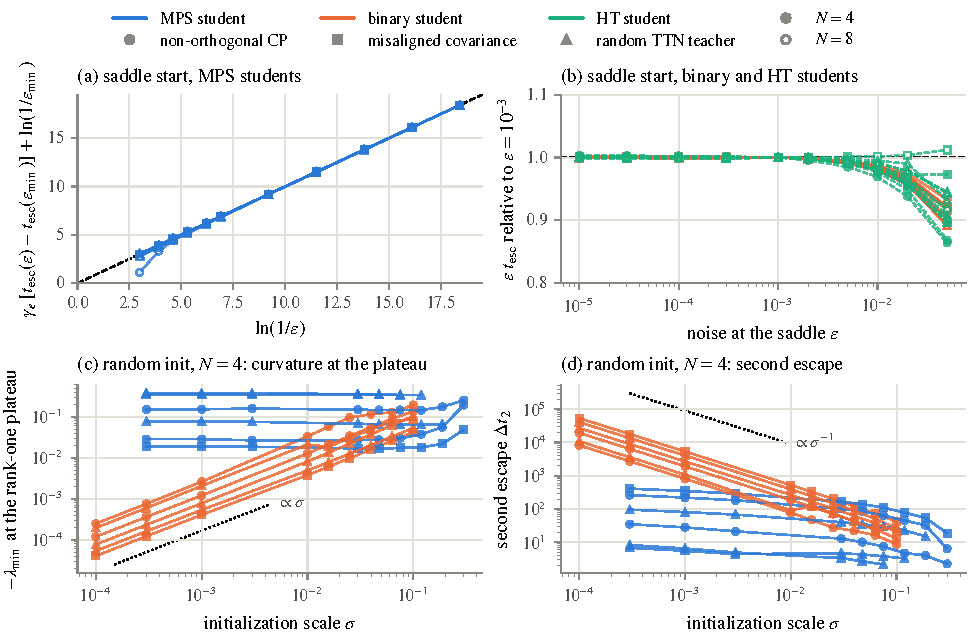
\includegraphics{data_teacher/contrast.pdf}
  \caption{One generic teacher, three trees. (a)~Saddle start, MPS students, 13 teachers: escape time
    rescaled by the predicted slope (mean over five seeds, $\gamma_e$ of the realized edge) against
    $\ln(1/\varepsilon)$; dashed: the prediction. (b)~Saddle start, binary and HT students, the same teachers
    except the misaligned one with $\Ns=8$, $\theta=20^\circ$: $\varepsilon\,t_{\rm esc}$ relative to its value at
    $\varepsilon=10^{-3}$ (per seed, then geometric mean); flat means $t_{\rm esc}\propto\varepsilon^{-1}$. (c),~(d)~Random
    initialization, the six teachers with $\Ns=4$ on MPS4 and binary4 (runs on the major rank-one saddle
    with a resolved plateau, geometric means over seeds): $-\lambda_{\min}$ of the gauge-projected Hessian at the
    plateau, and the second escape $\Delta t_2$. Takeaway: the same teachers give a strict saddle with a
    logarithmic escape at the predicted rate on the MPS, and a higher-order saddle
    ($\lambda_{\min}\propto\isc$, escape $\propto\varepsilon^{-1}$ or $\isc^{-1}$) on binary and HT trees.}
  \label{fig:dt-contrast}
\end{figure}

% ===========================================================================================
\subsection{Misaligned covariance}\label{sec:cov-misaligned}

The critical points, critical values and saddle types under a product covariance are those of the
whitened problem with teacher $\Sig^{1/2}\Wt$; escape rates are not, because the flow is preconditioned
\proven{} \newresult[for TTNs] (\cref{prop:A-precond}). With misaligned factors $\Sig^{1/2}\Wt$ is a
non-orthogonal CP teacher, with factors $\propto\Sigi i^{1/2}\fac ri$, while the escape is driven by $\Sig\Wt$, with
factors $\propto\Sigi i\fac ri$: the state must rotate after the escape, and misalignment alone can reverse the
order \derived{} \newresult{} (\cref{app:covariance}). Experiments \empirical{} ($d=\chi=4$, weights $(1,0.8)$,
$\beta\in\{0.5,1\}$, $\theta=0$--$45^\circ$, $\isc=0.05$ on binary4 and $0.1$ on MPS4, 20 seeds; an MPS4 sweep with $\beta=1$,
$\theta\in\{0,5,20\}^\circ$, nine $\isc$ from $3\cdot10^{-4}$ to $0.3$, ten seeds):
\begin{itemize}
  \item The first plateau is the predicted rank-one critical point of the $\Sig$-loss: median relative
    level errors $10^{-6}$--$10^{-3}$, median $\abs{\cos}\ge0.998$ with the critical tensor for $\theta\le30^\circ$, over
    the resolved plateaus (20--50\% of the MPS4 runs per $\theta$ have none at $\isc=0.1$).
  \item Early alignment with the race tensor (the best bond-rank-one approximation of $\Sig\Wt$), then
    realignment to the saddle \knownresult[in linear networks, binary4 being one:
    \citealp{atanasov2022neural}]: in $75$--$100\%$ of the binary4 runs at $\theta\ge10^\circ$, but on MPS4 only at
    $45^\circ$.
  \item Second escape on MPS4 (\cref{fig:dt-mps-laws}b) \newresult: $\isc^{-2.000}$ at $\theta=0$; at $20^\circ$ the log law
    (10 of 10 seeds) with slope $12.14\pm0.03$, below the bound $1/\abs{\lambda_{\min}}=12.31$ of its
    $\isc$-independent plateau curvature; at $5^\circ$ the log law (10 of 10) with $194.9\pm1.2$, approaching its
    bound $193.2$ from above (not yet asymptotic). The slope itself is not predicted: the head start under
    the preconditioned flow was not derived.
\end{itemize}

\begin{figure}[tbp]
  \centering
  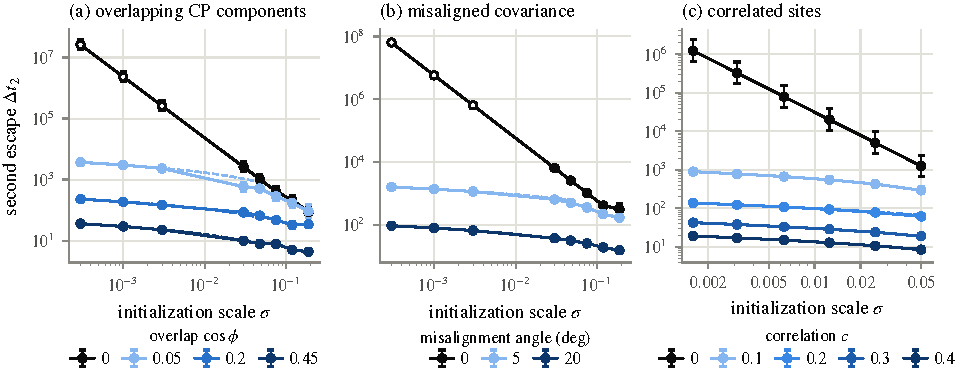
\includegraphics{data_teacher/mps_laws.pdf}
  \caption{MPS4 from random initialization: the second escape $\Delta t_2$ (onset events; runs on the major
    rank-one saddle with a resolved plateau; geometric mean over seeds with its standard error) when the
    teacher's components are made non-orthogonal in three ways. (a)~CP overlap $c$ ($d=4$, weights $(1,0.7)$,
    ten seeds); dashed: $h_e\ln(1/\isc)$ (\cref{cor:A-second-escape}), anchored at the smallest $\isc$ since the
    intercept is not predicted. (b)~Misaligned covariance at angle $\theta$ ($d=4$, ten seeds); dashed: slope
    $1/\abs{\lambda_{\min}}$, an upper bound. (c)~Correlated sites ($d=3$, four seeds); dashed: the two-stage law
    (\cref{app:covariance}; not computed for $\rho=0.1$, $0.3$). Black: the orthogonal baseline, dashed
    $\propto\isc^{-2}$; open markers: runs flagged by the float64-floor scan (dormant overlap $10^{-21}$--$10^{-12}$);
    without them the baseline exponents are $2.008\pm0.002$ ($c=0$) and $2.000\pm0.002$ ($\theta=0$). Takeaway: any
    non-orthogonality in the metric of the loss turns the $\isc^{-2}$ second plateau into a logarithmic
    one, with the predicted slope where there is a prediction.}
  \label{fig:dt-mps-laws}
\end{figure}

% ===========================================================================================
\subsection{Cross-site correlations}\label{sec:cov-correlated}

In the one-factor model $x^{(i)}=(1-\rho)^{1/2}z_i+\rho^{1/2}z_0$ (independent standard Gaussians; $\rho$ is the $c$
of \cref{app:covariance}) every site is whitened and two sites have covariance $\rho\Id$. The second-moment
matrix is not a product, so no whitening substitution exists; the loss is computed with the dense
matrix. The residual acquires \emph{pairing} tensors such as $(x^{(0)}\cdot x^{(1)})\,x^{(2)}_rx^{(3)}_r$, of bond
rank one on binary4 but $d$ on MPS4 \derived. On MPS4 the escape from the product saddle passes through
binary4's first plateau point, strict on MPS4 but of higher order on binary4, so the second plateau grows
by $\ln2\,[(1-\kappa_{\rm c})/\lambda_2+1/\lambda'']$ per halving of $\isc$: $2.128$ at $\rho=0.4$, $14.39$ at $\rho=0.2$ ($d=3$,
weights $(1,0.6)$) \derived{} \newresult{} (\cref{app:covariance}); binary4 stays at $\isc^{-1}$.
Experiments \empirical:
\begin{itemize}
  \item binary4 ($d=\chi=4$, weights $(1,0.7)$, $\isc=0.05$, 20 seeds): the first plateau falls from $0.33\,\Loss(0)$
    at $\rho=0$ to $0.29$, $0.20$, $0.14$, $0.10\,\Loss(0)$ at $\rho=0.2$--$0.5$, always at the predicted critical value
    (median relative error $\le5\cdot10^{-4}$): a blend with pairing terms, no longer a partial fit.
  \item Second escape \newresult{} (\cref{fig:dt-mps-laws}c; $d=3$, six $\isc$ from $0.0016$ to $0.05$, five seeds,
    events on the singular values across $01|23$): on MPS4 the log law in 4 of 4 seeds at every $\rho>0$ (seed 2 sits on
    the minor saddle and is excluded); increments per halving over the three smallest $\isc$ $2.133\pm0.003$
    at $\rho=0.4$ (predicted $2.128$) and $14.67\pm0.06$ at $\rho=0.2$ ($14.39$; $+2\%$, still falling), and
    $113.9\pm0.7$, $4.616\pm0.010$ at $\rho=0.1$, $0.3$ (no prediction computed); $\isc^{-2.000}$ at $\rho=0$. Binary4:
    $\isc^{-p}$, $p=1.005$--$1.011$. This repeats the theory's own check with more seeds: a replication, not
    an independent test.
  \item The MPS4 plateaus separate only logarithmically: separation ratio $2.6\to11$ at $\rho=0.4$ from
    $\isc=0.05$ to $0.0016$, against $14$--$19\to139$--$185$ on binary4.
  \item Online SGD (binary4, $\rho=0.3$, $\batch\ge256$, three seeds) crosses the same loss levels within $4\%$ of
    gradient flow.
\end{itemize}
HT students and $\Ns>4$ were not run with correlated inputs.

% ===========================================================================================
\subsection{Non-orthogonal CP teachers}\label{sec:teacher-cp}

The rank-one critical points are those of $g(x)=\ip{\bigotimes_ix_i}{\Wt}$ on unit rank-one tensors
\proven. With two components of equal weight and overlap $c$ at every site, an MPS has two rank-one
maxima (one near each component) iff $c<(\Ns-2)/\Ns$ and one blended maximum above \proven{} (among symmetric
points); unequal weights move the merger to a fold \derived; on binary4 the rank-one point is the top
singular pair of the $(01|23)$ matricization, a blend for every $c>0$ \newresult[elementary]
(\cref{prop:A-two-components}). The plateau is never a component. Experiments \empirical{} ($d=\chi=4$, weights
$(1,\tw2)$, $\tw2\in\{0.7,1\}$,
$c=0$--$0.8$, $\isc=0.05$ on binary4 and $0.1$ on MPS4, 20 seeds; an MPS4 sweep with $\tw2=0.7$,
$c\in\{0,0.05,0.2,0.45\}$, nine $\isc$ from $3\cdot10^{-4}$ to $0.3$, ten seeds):
\begin{itemize}
  \item MPS4 has two rank-one minima for $c\le0.45$ and one for $c\ge0.55$ ($\tw2=1$), two for $c\le0.35$ and
    one for $c\ge0.45$ ($\tw2=0.7$); binary4 one. First plateaus sit at these blends (median relative level
    errors $5\cdot10^{-5}$--$2\cdot10^{-3}$ on binary4, up to $3\%$ on barely resolved MPS4 plateaus; some binary4 runs
    with $\tw2=1$ sit at the second singular pair, a strict saddle), with levels falling as $c$ grows.
  \item Second escape on MPS4 (\cref{fig:dt-mps-laws}a) \newresult: $\isc^{-2.00}$ at $c=0$; for $c>0$ the log law (9 of
    9, 8 of 8, 8 of 8 seeds at $c=0.45$, $0.2$, $0.05$) with slopes $5.686\pm0.016$ ($h_e=5.682$), $34.40\pm0.20$
    ($34.14$) and $595\pm11$ ($570$; not yet asymptotic, as expected near the crossover overlap $c_\times=O(\isc)$
    of \cref{app:teachers}, a \conjecture), and an $\isc$-independent plateau curvature.
\end{itemize}
On binary4 the escape $\propto\isc^{-1}$ was measured for $c=0.2$ and $0.45$ only (\cref{sec:teacher-generic}).

% ===========================================================================================
\subsection{Random TTN teachers: plateaus are rank-constrained critical points}\label{sec:teacher-ttn}

With bond ranks fixed, the critical points are the fixed points of one-site alternating least squares
\proven{} \knownresult[in substance: \citealp{elden2011perturbation,holtz2012alternating}]
(\cref{prop:A-critical-points}); the hierarchical SVD is generically not one \proven{}
(\cref{prop:A-hsvd}). The
rank-one plateau should approach a local best rank-one approximation as $\isc^\alpha$, $\alpha=\min(\alpha_r,\alpha_a)$
(\conjecture: a heuristic crossing argument), and an MPS then gains rank bond by bond, first on
$e^*=\arg\max_e\sigma_2(M_e)$ with slope $h_{e^*}$ \derived. Experiments \empirical{} \newresult{} (MPS4 student,
$d=3$, $\chi=4$; five random MPS4 teachers with bond ranks $(2,3,2)$ and $\normF{\Wt}=1$; eight $\isc$ from
$10^{-3}$ to $0.2$; six seeds):
\begin{itemize}
  \item The rank-one plateau converges to the bond-rank-one critical point: per seed its distance
    falls as $\isc^\alpha$, $\alpha=0.72$, $0.83$, $0.41$, $0.93$, $0.80$ ($\pm0.01$--$0.03$), $0.07$--$0.15$ above the heuristic
    ($0.64$, $0.68$, $0.34$, $0.80$, $0.72$) for every teacher. For three teachers it is separated from every
    SVD-type truncation (hierarchical SVD, TT-SVD in both directions): at $\isc=10^{-3}$ it lies
    $10^{-4}$--$2.5\cdot10^{-3}$ from the critical point and $1.5\cdot10^{-3}$--$0.028$ from the nearest truncation
    (relative to $\normF{\Wt}$). For the other two teachers, and at the higher-rank plateaus, the critical
    point lies within $0.0032$ of an SVD-type truncation and the plateaus do not discriminate between them.
    (In CP factorization, small initialization follows a rank-one trajectory, \citealp{razin2021implicit}.)
  \item Ranks grow one bond at a time, e.g.\ $(1,1,1)\to(2,1,1)\to(2,2,1)\to(2,3,1)\to(2,3,2)$. The first increase
    after the rank-one plateau follows the log law in 26 of 26 seeds, with single-route slopes within
    $0.3$--$1.6\%$ of $h_{e^*}$ (e.g.\ $5.188\pm0.008$ against $5.175$), always on $e^*$ at $\isc=10^{-3}$; later increases
    were not timed. Gradient descent on tensor-train completion shows a plateau followed by abrupt
    rank growth \citep{milanesi2021implicit}.
\end{itemize}

% ===========================================================================================
\subsection{Teacher and student on different trees}\label{sec:teacher-mismatch}

A student bond must reach the rank of the teacher's matricization across it, bounded by products of
bond dimensions over cuts of the teacher's tree \proven{} \knownresult[standard min-cut bound; cf.\
\citealp{grasedyck2011introduction}, Lemmas~7--8] (\cref{app:teachers}):
a binary8 student of an MPS8 teacher of bond rank $r$ needs rank $\min(d^2,r^2)$ on the bonds of sites
$\{2,3\}$ and $\{4,5\}$. The routes give \emph{bottom-up order} \derived{} \newresult: the root bipartition
$\{0123\}|\{4567\}$ (the teacher's middle bond) has a three-core route only after both halves have bond
rank above one below it, so it grows only after a bottom bond on each half, whatever its teacher
Schmidt value. Experiments \empirical{} \newresult{} (binary8 student, $\chi=4$, twelve random MPS8 teachers
with bond ranks 2, $\isc=0.3$, $0.4$, $0.5$, eight seeds): in the 7 teachers whose root cut has a larger
teacher Schmidt value than both bottom bonds of a half, so that a weight order disagrees, bottom-up
order holds in 163 of 168 runs (56 of 56 at $\isc=0.3$), including 117 of 120 for five teachers whose root
cut is the strongest of all by $5.5$--$13\%$; the 5 exceptions grow the root after a bottom bond on one half
only. Over all 12 teachers: 249 of 256. ``Largest teacher Schmidt value first'' fails, and ``a sibling
pair first'' is no rule (8--100\% of the runs by teacher). Scope: $\Ns=8$, $\isc=0.3$--$0.5$. (An MPS8 student of
binary8 teachers at $\isc=0.45$ grows the predicted bond first in 2 of 24 runs; with $\ln(1/\isc)=0.8$ this is no
test of the asymptotic race of \cref{prop:A-agf-race}.)

% Summary table of Sec. 6.10, placed here so that it floats into the section.
\begin{table}[t]
  \centering
  \caption{Input covariance and teacher structure: what changes, and what predicts it. ``Escape'': the
    escape from the rank-one saddle.}
  \label{tab:cov-summary}
  \footnotesize
  \begin{tabularx}{\textwidth}{@{}>{\raggedright\arraybackslash}p{2.7cm}>{\raggedright\arraybackslash}X
      >{\raggedright\arraybackslash}p{4.0cm}@{}}
    \toprule
    complication & what changed (\empirical) & predicted by \\
    \midrule
    aligned covariance & quantitative only: order and times follow $\Lambda_r\tw r$, plateaus and swaps
      $\Lambda_r\tw r^2$; exponents unchanged & whitened problems with $\Lambda\tw{}$ (race) and $\Lambda^{1/2}\tw{}$
      (landscape) \\
    generic teachers & escape strict and logarithmic on MPS ($\le0.4\%$ from the saddle, $\le1.3\%$ from random
      init); $\propto\varepsilon^{-1}$, $\isc^{-1}$ on binary and HT & two-core routes and their rates \\
    misaligned covariance & plateaus at critical points of the $\Sig$-loss; early alignment (binary4); MPS4
      escape logarithmic & $\Sig^{1/2}\Wt$; slope only bounded \\
    cross-site correlations & binary4: first saddle with pairing terms; MPS4: logarithmic two-stage
      escape & two-stage law (replication) \\
    overlapping CP components & blended plateaus; MPS4 rank-one maxima merge at $c=1/2$; logarithmic
      escape & rank-one landscape; $h_e$ within $1\%$ ($c\ge0.2$) \\
    random TTN teachers & plateaus at rank-constrained critical points (3 of 5 teachers separated from
      SVD truncations); ranks grow bond by bond & critical points; $h_{e^*}$ within $1.6\%$ \\
    teacher on another tree & bottom-up order on binary8 (163 of 168 discriminating runs) & routes \\
    star teachers & larger learned component left iff $\lambda_{\max}(\Gamma)>\tw q$; log time on MPS4, polynomial
      on HT4 & piggyback graph; rates within $0.2\%$ \\
    real data & pending (\cref{sec:real-data}) & -- \\
    \bottomrule
  \end{tabularx}
\end{table}

% ===========================================================================================
\subsection{Star teachers: forgetting a learned component}\label{sec:teacher-star}

A learned component $j$ without a two-core route to the rest is a strict saddle iff
$\lambda_{\max}(\Gamma)>\tw j$, $\Gamma$ the weighted adjacency matrix of the piggyback graph, and then
$\lambda_{\min}=-q_j^{\Kc-2}(\lambda_{\max}(\Gamma)-\tw j)$ \proven{} \newresult[for general trees; deep linear networks:
\citealp{achour2024loss}, Thm~7] (\cref{prop:A-piggyback-graph}). The \emph{star} has $q=0000$ ($\tw q=2$) and
$r=1010$, $r'=1001$ (weight $w$ each, $d=2$), which share the piggyback node: $\lambda_{\max}(\Gamma)=\sqrt2\,w$, so
``$q$ learned'' ($\params_q$) is strict iff $w>\sqrt2$, although both residual components are smaller and each
needs three or more cores. Experiments ($\chi=3$; MPS4, binary4, HT4; saddle start at $\params_q$ with
$\varepsilon=10^{-6}$--$10^{-2}$, five seeds; random initialization at $w=1.2$, $1.6$, ten seeds):
\begin{itemize}
  \item \emph{Hessian} \proven{} and computed: the formula holds to $10^{-15}$ on MPS4, binary4, HT4 and a
    binary8 analogue ($-0.3716$, $-0.3310$, $-0.4311$, $-0.4311$ at $w=1.6$); no negative eigenvalue for $w\le1.40$.
    This repeats the theory's check; binary4 is a deep linear network, where it is known.
  \item \emph{Threshold} \empirical{} \newresult[dynamics]: at $\varepsilon=10^{-6}$ no seed leaves $\params_q$ at
    $w=1.4138$ ($\lambda_{\max}(\Gamma)/\tw q=0.9998$) and all do at $1.4146$ ($1.0003$), on MPS4 and binary4; on HT4
    the step lies between $1.40$ and $1.42$ for $\varepsilon\le10^{-3}$. At $\varepsilon=10^{-2}$ it moves to $1.43$--$1.44$: near the
    threshold the strict escape is slow and the polynomial route that adds $r$ wins at moderate noise.
  \item \emph{One or two strict stages} \derived{} (from the computed Hessians) and \empirical{}
    \newresult: the slope of the escape time against $\ln(1/\varepsilon)$ is $1/\abs{\lambda_q}$ within $0.21\%$ where the
    event times one strict stage ($w\ge1.48$ on all trees, every $w$ on binary4). Near the threshold on MPS4
    the flow stops at a blended rank-one point that keeps $\ov q=0.98$, $0.93$ ($w=1.42$, $1.44$) and is itself
    strict: the measured $130.0\pm0.2$ and $29.39\pm0.02$ equal $1/\abs{\lambda_q}+1/\abs{\lambda_b}=129.9$ and $29.3$ (one stage:
    $86.4$, $19.4$). On HT4 that point has no negative eigenvalue, and leaving it takes a time $\propto\varepsilon^{-1}$
    ($p=0.995$, $0.998$; at $w=1.6$, $\ov q<\frac12$ after $3.4\cdot10^3$, $3.3\cdot10^4$, $3.3\cdot10^6$ for $\varepsilon=10^{-3}$, $10^{-4}$,
    $10^{-6}$). A star forgets $q$ in logarithmic time on MPS4 and binary4 but polynomially on HT4: the tree
    contrast of \cref{sec:teacher-generic} again.
  \item \emph{Random initialization} \empirical{} \newresult{} ($w=1.6$; $\isc=0.01$--$0.1$ on MPS4, $0.005$--$0.05$ on
    binary4):
    the flow never sits at $\params_q$ (at most $0.13$ time units at its loss level, one seed $1.7$; up to 538
    at ``$q$ forgotten''). The initialization direction sets the class: $q$ learned last (binary4 7 of 10
    seeds, MPS4 1 of 10), $\ov q$ rising to $0.78$--$1.00$ and decaying (3, 4 of 10), or a blended start with
    $\ov q\le0.68$ (MPS4, 5 of 10). The decay deepens steeply as $\isc$ decreases, not as a power law; $q$ is
    relearned last. Sub-critical stars ($w=1.2$) keep $q$ ($\min\ov q\ge0.992$).
\end{itemize}
\emph{Withdrawn:} the laws $\min\ov q\propto\isc^{5.7\pm0.3}$ and a relearning time $\propto\isc^{-1.4}$ from random
initialization; they pooled two classes of runs, dropped the points where $\ov q$ crosses zero, and
describe runs that never visit $\params_q$.

% ===========================================================================================
\subsection{Real data}\label{sec:real-data}
\placeholder{To be written when the real-data experiment (PLAN.md B5: MNIST with quadtree, MPS and
scrambled-site trees) is finished.}
% TODO(real-data): another agent writes this subsection. Question: which of the effects above survive
% real inputs (non-Gaussian, correlated pixels, unknown teacher): the plateau structure and its scaling
% with sigma, the order of bond-rank growth, and the dependence on the tree (quadtree vs MPS vs
% scrambled sites). Settings go to Appendix B and figures to Appendix C, as for the other experiments.

% ===========================================================================================
\subsection{Summary}\label{sec:cov-summary}

Only the aligned covariance leaves the qualitative picture unchanged (\cref{tab:cov-summary}). Every
other complication breaks the orthogonality of the teacher's components in the metric of the loss, and
then the student's tree decides whether the escape from the rank-one saddle is logarithmic (MPS) or
polynomial (binary, HT). The baseline theory predicts each change after the substitution in the
table, except the slope under a misaligned covariance from random initialization, which is only
bounded.

% sections/07_open_questions.tex -- Open questions. SKELETON.
\section{Open questions}\label{sec:open}

\placeholder{Skeleton. Questions left open by this work, each with what would settle it.}
% TODO: collect from sections 3-6 and the agents' "open problems". Candidates from PLAN.md:
%  - Full saddle sequence for random init (a TTN analogue of the DLN conjecture of Jacot et al.
%    2021 and of the explicit algorithm for diagonal networks of Pesme & Flammarion 2023): is the
%    sequence determined by an algorithm on the teacher and the tree?
%  - Rigorous version of the escape-time formula (directional convergence + radial growth) and of
%    the locality rule H2 / saddle-type rule H3.
%  - Distribution of the learning order for tensorial teachers (basins of the spherical flow of
%    g = <W, W*>), including its dependence on chi and d.
%  - Infinite-bond-dimension limits: is there a muP-type limit with feature learning for TTNs, and
%    what is its dynamics?
%  - Beyond product inputs and multilinear features; classification / multi-output.
%  - Practical consequences: initialization and tree choice for TN learning.


\bibliography{references}

\appendix
% sections/A_derivations.tex -- Appendix A: derivations. SKELETON.
% Each derivation: assumptions, statement, proof or derivation, status tag, and the testable
% prediction it feeds into (with a pointer to the figure that tests it). Sources: the theory notes
% notes/theory_escape.md, notes/theory_saddles.md, notes/theory_regimes.md and the agents' notes.
\section{Derivations}\label{app:derivations}

\placeholder{Skeleton. Full derivations behind the statements of the main text; the short proofs of
\cref{sec:setup} are not repeated.}

\subsection{Gradients and the tangent kernel of a TTN}\label{app:gradients}
\placeholder{Environment formula for $\nabla_{\G{v}}\Loss$; the tangent kernel at initialization and
its scale $\isc^{2(\Kc-1)}$.}
% TODO: grad_{G_v} L = contraction of the residual Sigma(W - W*) with all cores except G_v (the
% environment of v); expected kernel at fan-in init; needed for Sec. 5.1 (lazy time rescaling).

\subsection{Escape from the origin}\label{app:escape}
\placeholder{Spherical flow and radial growth for the degree-$\Kc$ homogeneous correlation
$g(\params)=\ip{\W(\params)}{\Wt}$; alignment time; the first-escape formula of
\cref{sec:s2s-escape}.}
% TODO(theory_escape): near the origin, dynamics ~ gradient flow of g. With d tau = |theta|^{K-2} dt
% the direction follows the spherical gradient flow of g and the radius grows like
% exp(K int g). Result to state: t_1 ~ rho_0^{-(K-2)} [tau_align + K^{K/2-1}/((K-2) s_1)];
% aligned limit a_0^{-(K-2)}/((K-2) s). State assumptions (separation of time scales, nondegenerate
% local maxima of g on the sphere). Status: \derived.

\subsection{Expansion around a learned-component saddle}\label{app:saddles}
\placeholder{Second-order expansion of $\Loss$ in the directions that add a new component; the
locality rule for $k$ and the saddle type.}
% TODO(theory_saddles): lowest-degree escape route; reduced ODE for its amplitude; k-rule (H2) and
% strict-iff-k=2 (H3); gauge projection of the Hessian (orbit tangents of eq:gauge).

\subsection{Correction of a wrong learning order}\label{app:piggyback}
\placeholder{The ``piggyback'' direction and its Hessian eigenvalue $q(\tw{\mathrm{learned}}-
\tw{\mathrm{new}})$ (hypothesis H1b).}
% TODO: hand derivation for the N = 4 binary tree with odeco teacher, balanced learned amplitudes
% q = s^{1/K}; generalize.

\subsection{Gradient-descent stability limit}\label{app:gd-stability}
\placeholder{Sharpness at the balanced global minimum and the predicted $\lr_{\max}$.}
% TODO: PLAN.md guess eta_max ~ 2 / (K s_1^{2 - 2/K}): verify (for one balanced mode the Hessian
% of 1/2 (s - prod_v q_v)^2 at q_v = s^{1/K} is s^{2-2/K} 1 1^T, top eigenvalue K s^{2-2/K}) or
% correct it for the full TTN.

\subsection{Regime boundaries}\label{app:boundaries}
\placeholder{Lazy criterion and saddle-to-saddle separation criterion as functions of $\isc$,
$\chi$, $\Kc$ and imbalance; large-bond-dimension scalings.}
% TODO(theory_regimes): Chizat-type criterion; S2S boundary from escape times with separation
% ratio 3; muP-type per-core scalings from the spectral condition.

% sections/B_experimental_details.tex -- Appendix B: experimental details. SKELETON.
% One subsection per experiment folder. Pull the numbers from the experiment READMEs and configs
% (experiments/<name>/configs/*.yaml); never retype them by hand if a script can print them.
\section{Experimental details}\label{app:experiments}

\placeholder{Skeleton. For every experiment: trees, dimensions, teachers, initialization, dynamics
and tolerances, sweeps, seeds, time budgets, compute cost.}

\subsection{Common settings}\label{app:exp-common}
\placeholder{Double precision; Dormand--Prince 5(4) with relative and absolute tolerances
$10^{-8}$ and $10^{-12}$ unless stated; recording grid; conservation-drift threshold $10^{-6}$;
event detection; Hessian and kernel computations.}
% TODO: how crossing times are located (interpolation on the log grid vs dense output / root
% finding as in experiments/pilot_h2_locality/h2sim.py); Hessian by autodiff + gauge projection;
% probe set seed; machines used (vCPU type), wall times, total cost from notes/spend.md.

\subsection{Saddle-to-saddle experiments}\label{app:exp-s2s}
\placeholder{Settings of the experiments of \cref{sec:s2s} (s2s-core, locality, order).}
% TODO: table per experiment: trees, N, d, chi, teacher (type, weights), sigma grid, seeds, t_max,
% loss floor, number of runs, cost.

\subsection{Regime-map experiments}\label{app:exp-regimes}
\placeholder{Grids, seeds and time budgets of the phase diagrams of \cref{sec:regime-map}.}

\subsection{Covariance and teacher experiments}\label{app:exp-data-teacher}
\placeholder{Settings of \cref{sec:covariance-teacher}.}

\subsection{Optimizer and sample-size experiments}\label{app:exp-optim}
\placeholder{Learning rates, batch sizes, training-set sizes and seeds of \cref{sec:other-optim}.}

\subsection{Optimizers used in practice}\label{app:exp-optimizers}
Settings of \cref{sec:other-optimizers}. Experiment folder \path{experiments/optimizers/} (one YAML
configuration per sweep in \path{configs/}); findings and claims withdrawn after review in
\path{notes/optimizers.md}, sections 2, 3 and 5.

\paragraph{Problems.}
Whitened Gaussian inputs, exact population loss (empirical loss in the finite-sample sweep), double
precision. Teacher seed 100; initialization seeds 0--5, from a stream independent of the teacher's.
\begin{itemize}
  \item \emph{binary4}: binary tree, $\Ns=4$ ($\Kc=3$), $d=3$, $\chi=4$; odeco teacher with weights
    $(3,2,1)$ and Haar-random site bases.
  \item \emph{binary8}, \emph{MPS8}: $\Ns=8$ ($\Kc=7$ and $8$), the same odeco teacher, $d=3$, $\chi=4$.
  \item \emph{E8} on binary8 and MPS8: pattern teacher with $d=2$, $\chi=3$ and patterns
    $\pi_0=(1,\dots,1)$ (weight $1$), $\pi_A$ equal to $2$ at sites 4 and 5 (weight $0.4$) and
    $\pi_B$ equal to $2$ at sites 2 and 7 (weight $0.7$), $1$ elsewhere. The cores that carry the
    differing sites span $k=2$ ($\pi_A$) and $k=6$ ($\pi_B$) cores on the MPS and $k=5$ for both on
    the binary tree.
\end{itemize}

\paragraph{Initializations.}
Fan-in \eqref{eq:init} with per-core scale $\isc$; \emph{balanced}: the same $\Wz$ in the gauge with
$\Q e=0$ on every edge. All deep-tree baselines use the balanced version, because fan-in gradient flow
converges by $t=2\cdot10^6$ in none of the 12 MPS8 odeco runs (the conservation-law trap of
\cref{prop:A-trap}, verified at the route ends in 11 of the 12 stalls), against 10 of 12 (binary8
odeco), 11 of 12 (binary8 E8) and 11 of 12 (MPS8 E8) fan-in runs. Methods whose iterates depend on the
gauge were run from both versions; re-gauged GD, Riemannian GD, ALS and DMRG depend only on $\Wz$
and were run from the balanced one.

\paragraph{Dynamics.}
All methods stop at $\Loss<10^{-6}\Loss_0$ (finite samples: empirical loss below $10^{-8}$ times its
initial value) or at their budget.
\begin{itemize}
  \item \emph{Gradient flow}: SciPy LSODA with relative and absolute tolerances $10^{-9}$ and
    $10^{-14}$ and the exact Hessian as Jacobian (Radau as fallback), instead of the default
    integrator of \cref{sec:setup-dynamics}; the crossings $\ov r\in\{0.1,0.5,0.9\}$ are located by
    root finding, so event times are exact. Budgets: $t_{\max}=8/\isc$ (binary4), $2\cdot10^6$
    (deep trees), $4\cdot10^6$ (binary8 scan), $10^6$ (finite samples).
  \item \emph{GD and heavy ball} (PyTorch): $\lr=0.02$ and $0.002$ with $\beta=0.9$ on binary4
    ($0.13\,\lr_c$ for both, counting heavy ball's effective step $\lr/(1-\beta)$); $\lr=0.01$ and
    $0.001$ on the deep trees ($0.23$--$0.27\,\lr_c$), at $\isc=0.8$ only, because gradient-flow
    plateaus at $\isc=0.3$ last $10^4$--$10^6$ time units. Budgets $8/\isc$ (binary4) and $2\cdot10^4$
    (deep) gradient-flow time units, at most $5\cdot10^5$ steps.
  \item \emph{Adam} (PyTorch, bias-corrected): $\beta_1=0.9$, $\beta_2=0.999$ (also $0.99$ and $0.9$
    at $\lr=10^{-3}$ on binary4), $\epsilon=10^{-8}$ ($10^{-30}$ in the $\epsilon$ sweep),
    $\lr\in\{10^{-4},3\cdot10^{-4},10^{-3},10^{-2}\}$ on binary4 and $\{10^{-3},10^{-2}\}$ on the deep
    trees. \emph{RMSProp}: $\alpha=0.99$, $\epsilon=10^{-8}$, $\lr\in\{10^{-4},10^{-3}\}$. Budgets
    $10^5$--$3\cdot10^5$ (binary4), $3\cdot10^5$ (deep), $5\cdot10^5$ (binary8 scan) and $2\cdot10^5$
    ($\epsilon$ sweep) steps.
  \item \emph{Re-gauged GD}: $\lr=0.02$ (binary4) and $0.01$ (deep); QR sweeps from the leaves to
    the root bring the cores to the root-centred canonical form every 1 or 50 steps; $5\cdot10^4$,
    $10^5$ and $2\cdot10^5$ (binary8 scan) steps.
  \item \emph{Riemannian GD}: $\lr\in\{0.1,1\}$; tangent projection by least squares with the dense
    Jacobian of $\W(\params)$ (relative cutoff $10^{-12}$), so only small $d^\Ns$ are feasible;
    leaves-to-root HSVD retraction; 2000 steps.
  \item \emph{Gram-preconditioned GD}: $\lr\in\{0.01,0.1,0.5\}$; each Kronecker factor of a core's
    Hessian block is damped by $10^{-3}$ times its mean eigenvalue (scale-free) or, at $\lr=0.1$, by
    an absolute floor $10^{-4}$ or $10^{-2}$; no divergence guard, because the first step overshoots
    by up to $10^{34}\Loss_0$ before the loss returns; $5\cdot10^4$ (binary4; $2\cdot10^5$ with a
    floor) and $10^5$ (deep) steps.
  \item \emph{ALS} (one site) and \emph{DMRG} (two sites, then SVD truncation to at most $\chi$
    values with relative cutoff $10^{-12}$): exact least squares; the orthogonality centre moves by QR
    along a depth-first tour of the tree; at most 50 sweeps.
\end{itemize}

\paragraph{Sweeps and run counts.}
\Cref{tab:exp-optimizers} lists the sweeps; six initialization seeds per setting, 2529 runs in total.

\begin{table}[ht]
  \centering
  \caption{Sweeps of the optimizer experiment (\cref{sec:other-optimizers}), one configuration file
    per sweep in \texttt{experiments/optimizers/configs/}.}
  \label{tab:exp-optimizers}
  \footnotesize
  \begin{tabularx}{\textwidth}{@{}>{\raggedright\arraybackslash}p{2.9cm}
      >{\raggedright\arraybackslash}p{2.7cm}>{\raggedright\arraybackslash}p{2.5cm}X r@{}}
    \toprule
    sweep & problem & $\isc$ & methods & runs \\
    \midrule
    \texttt{scaling\_b4} & binary4, fan-in & $0.002\cdot2^j$, $j=0,\dots,6$ & 19 settings: gradient flow,
      GD, heavy ball, Adam (6), RMSProp (2), re-gauged GD (2), Riemannian GD (2), Gram (2), ALS, DMRG
      & 798 \\
    \texttt{precond\_b4} & binary4, fan-in & as above & Gram: 3 step sizes with scale-free damping,
      2 absolute floors & 210 \\
    \texttt{deep} & binary8, MPS8; odeco, E8; balanced and fan-in & $0.3$, $0.8$ & gradient flow, GD
      and heavy ball ($\isc=0.8$), Adam (2), RMSProp, Gram; from the balanced $\Wz$ only: re-gauged GD
      (2), Riemannian GD (2), ALS, DMRG & 864 \\
    \texttt{later\_b8} & binary8 odeco, balanced & $0.25$, $0.3$, $0.35$, $0.4$, $0.5$, $0.6$, $0.8$ &
      gradient flow, Adam (2; every step recorded for the first 2000 steps), re-gauged GD & 168 \\
    \texttt{eps\_mps8} & MPS8 odeco, balanced & $0.01$, $0.015$, $0.02$, $0.03$, $0.05$, $0.1$,
      $0.2$, $0.3$ & Adam: $\lr\in\{10^{-3},10^{-2}\}$, $\epsilon\in\{10^{-8},10^{-30}\}$ & 192 \\
    \texttt{implicit\_bias2\_b4} & binary4, $\nsamp\in\{45,60\}$, data seeds 200--203 & $0.01$,
      $0.1$ & gradient flow, Adam (2); pairs share draw and initialization & 288 \\
    \texttt{adam\_probe} & binary4, binary8, MPS8 E8 & single runs & Adam and RMSProp internal state
      (illustration only) & 9 \\
    \bottomrule
  \end{tabularx}
\end{table}

\paragraph{Events and classification.}
\begin{itemize}
  \item Event $r$ is the last upward crossing of $\ov r=\frac12$ after which $\ov r$ stays at least
    $\frac12$; transient crossings, which the first-crossing rule of \cref{sec:setup-diagnostics}
    would count, are not events. Width: final rise from $0.1$ to $0.9$. Saddle-to-saddle: every
    separation ratio $\sep i>3$ (\cref{tab:regimes}).
  \item Discrete methods record loss and overlaps at every step for the first 2000 steps, then every
    $\max(1,n_{\rm steps}/(5\cdot10^4))$ steps. A first escape or gap shorter than two recording
    intervals is unresolved and excluded from fits (and counted in the result tables). Two components
    that cross $\frac12$ in the same step or micro-step have no resolved order. For Gram-preconditioned
    GD, events are defined only after the loss has returned below $\Loss_0$; a component already above
    $\frac12$ at that point has no resolved event.
  \item Exponents: per seed, a least-squares fit of $\ln T$ against $\ln\isc$ over the $\isc$ at which
    the seed follows its most common learning order (for plateau durations, not for times to reach a
    loss level); mean $\pm$ standard error over seeds. A logarithmic law fitted in the same space
    serves as comparison (gradient flow on binary4: root-mean-square residual of $\ln T$ $0.005$ for
    the power law, $0.62$ for the logarithmic law).
  \item Orders are compared with gradient flow only where both are resolved, for the same problem,
    $\isc$ and seed. Re-gauged GD, Riemannian GD, ALS and DMRG give one trajectory per seed at every
    $\isc$, so their orders are counted over the six independent seeds (at the smallest $\isc$).
  \item \emph{$\epsilon$ test} \eqref{eq:adam-eps}: $T_{\rm GF}(\isc)$ is the seed's exact
    gradient-flow first-escape time at $\isc=0.3$ (\texttt{deep} sweep, same balanced initial point
    up to scale) times $(0.3/\isc)^6$, and $n_{\rm sign}$ the median over $\isc$ of the same seed's
    escape with $\epsilon=10^{-30}$ at the same $\lr$. Runs without an escape within $2\cdot10^5$ steps
    enter only through the check that the prediction exceeds the budget.
  \item Convergence for cost and time-to-loss tables: $\Loss<10^{-3}\Loss_0$. Runs that hit their budget
    are reported as budget-limited, never as stalls. RMSProp hovers above $10^{-6}\Loss_0$ on the deep
    trees within $3\cdot10^5$ steps; its events are used, its convergence flags are not.
\end{itemize}

\paragraph{Excluded runs.}
Runs replaced after review round 1 are kept in \path{superseded/} subfolders of the raw data and
ignored by the analysis: gradient-flow runs whose event times were interpolated on an output grid
(errors up to $1.7\%$), Gram-preconditioned runs stopped by a $10^6\Loss_0$ loss guard after one step,
binary8 Adam runs recorded only every 10 steps, and the first finite-sample sweep
(\texttt{implicit\_bias\_b4}, 288 runs, one data draw per initialization). The pilots
(\texttt{pilot\_calib}, \texttt{pilot\_trap}) support no claim. Raw trajectories (one file per run,
2.2\,GB) are not in the repository; \cref{app:reproducibility} says how to regenerate them.

% sections/C_reproducibility.tex -- Appendix C: reproducibility. SKELETON (structure is final).
% Keep the figure table in sync with report/figures.txt: every figure included in the report has
% one row here and one line there.
\section{Reproducibility}\label{app:reproducibility}

\placeholder{Skeleton. How every number and figure in this report is regenerated.}

\subsection{Software and data}\label{app:repro-software}
\placeholder{Repository layout, environment and where raw outputs live.}
% TODO: uv project, Python 3.13, PyTorch (version from uv.lock), double precision; shared library
% ttn/ with tests (uv run pytest); one folder per experiment with README, configs/, code and
% results/ (small summary data and figures, in git); raw trajectories in data/<experiment>/ (not in
% git; each experiment README says how to regenerate them). Give the git commit of the report
% build.

\subsection{Figures}\label{app:repro-figures}
\placeholder{Table: figure, experiment folder, script and command, config, raw data needed.}
% TODO: one row per figure, e.g.
%   Fig. x | experiments/s2s_core | uv run python experiments/s2s_core/plot_escape.py | configs/... |
%   data/s2s_core/... (regenerate with ...).
% Figures are copied into report/figures/ by report/collect_figures.sh from the list in
% report/figures.txt; the TikZ figure of Sec. 2 is drawn from report/tikz/trees.tex.

\subsection{Building the report}\label{app:repro-build}
The report is built by \path{report/build.sh} (pdflatex, BibTeX, then pdflatex until the
cross-references are stable), after \path{report/collect_figures.sh} has copied the figures listed
in \path{report/figures.txt} from \path{experiments/*/results/} into \path{report/figures/}.
\path{report/README.md} describes both scripts.


% Appendix D collects material moved out of the main text (one file per main section; see notes/report_style.md).
\section{Supplementary results}\label{app:supp}
Material moved here from the main text: detailed tables, secondary checks, and the provenance and corrections
of each result after review.
\InputIfFileExists{sections/D_s2s}{}{}
\InputIfFileExists{sections/D_regimes}{}{}
\InputIfFileExists{sections/D_optim}{}{}
\InputIfFileExists{sections/D_covariance}{}{}

\end{document}
